\documentclass{report}
\usepackage[a4paper, total={6in, 8in}]{geometry}
\usepackage{listings}
\usepackage[utf8]{vietnam}
\usepackage{pgfplots}
\usepackage[shortlabels]{enumitem}


\usetikzlibrary{arrows}
\usepgfplotslibrary{polar}
\usepgflibrary{shapes.geometric}
\usetikzlibrary{calc}

\pgfplotsset{compat=1.18}

\usepackage{hyperref}
\hypersetup{
    colorlinks,
    citecolor=black,
    filecolor=black,
    linkcolor=blue,
    urlcolor=blue
}

\title{Giải \& diễn đạt bài tập Kinh tế học đại cương Đại học Thăng Long theo cách dễ hiểu hơn
}
\author{Tác giả: Lê Hoàng Long \\ Email: \href{mailto:hoanglong1712@gmail.com}{hoanglong1712@gmail.com} 
\\ Số điện thoại: \textcolor{blue}{(+84) 0359568862} 
hoặc \textcolor{blue}{(+84) 0359480290} \\
Danh sách các video hướng dẫn giải bài tập đi kèm tài liệu này \\
 \url{https://www.youtube.com/playlist?list=PLIpLw6v7Z1ql_ME2f8F7q4CN38vdjqskw} \\
 Địa chỉ GitHub chứa các tài liệu liên quan : 
 \\ 
 \url{https://github.com/hoanglong1712/kinh-te-hoc-dai-cuong-dai-hoc-thang-long-2021}
 }
\date{ }

\begin{document}

\maketitle

\tableofcontents

\setcounter{chapter}{2}
\chapter{CÁC LỰC LƯỢNG 
CUNG CẦU TRÊN THỊ 
TRƯỜNG}

\section{Điều gì xảy ra với giá và lượng cân bằng trên thị trường máy lạnh trong các
  tình huống sau:}

\begin{enumerate}[(a)]
    \item Thời tiết trở lên nóng bất thường, người bán không thay đổi lượng bán ra.
    \item  Lượng máy lạnh nhập khẩu gia tăng
    \item  Giá điện tăng cao, người bán không thay đổi lượng bán ra.
    \item  Các nhà khoa học khuyến cáo, máy lạnh có hại cho sức khỏe.
    \item  Thu nhập của người tiêu dùng giảm mạnh do suy thoái kinh tế.
    \item  Nhiều doanh nghiệp rời bỏ thị trường do chính phủ tăng thuế.
    \item  a và b xảy ra đồng thời nhưng ảnh hưởng của a mạnh hơn.
    \item  e và f xảy ra đồng thời
\end{enumerate}

\section{Cung – cầu về sản phẩm Y có dạng: $Q_S = 2P - 8$ và $Q_D = 15 - 0.5P$
  (trong đó Q tính bằng triệu tấn, P tính bằng nghìn đồng/tấn)}

\begin{enumerate}[(a)]
    \item Xác định giá và sản lượng cân bằng của sản phẩm Y.
    \\
    $Q_S = Q_D$
    \\ 
    $2P - 8 = 15 - 0.5P$
    \\
    $2.5P = 15 + 8 $
    \\
    $2.5P = 23$
    \\ 
    $P = 9.2$
    \\
    $Q_S = Q_D = 10.4$

    \begin{tikzpicture}
        \draw [->] (0,0) -- (5,0)node[right] {$Q$};
        \draw [->] (0,0) -- (0,5)node[above] {$P$};
        \draw[scale = 0.1, domain=0:20, smooth, variable=\x, color=blue] plot ({\x}, {\x /2 + 4});
        \draw[scale = 0.1, domain=0:20, smooth, variable=\x, color=red] plot ({\x}, {30 - 2 * \x});
        \filldraw[scale = 0.1, color=purple] (10.4, 9.2) circle (5pt) node[anchor=west]{A (10.4, 9.2)};
    \end{tikzpicture}

    \item Vì một lý do nào đó lượng cầu giảm 1 triệu tấn ở mọi mức giá, khi đó giá và lượng thay
          đổi như thế nào. Vẽ đồ thị minh họa câu a và câu b trên cùng một đồ thị
    \\ giá giảm , lượng cũng giảm
    \\
    cũ $Q_D = 15 - 0.5P$ 
    \\
    mới $Q_D = 14 - 0.5P$
    \\
    \begin{tikzpicture}
        \draw [->] (0,0) -- (5,0)node[right] {$Q$};
        \draw [->] (0,0) -- (0,5)node[above] {$P$};

        \draw[scale = 0.2, domain=0:20, smooth, variable=\x, color=green] plot ({\x}, {28 - 2 * \x});

        \draw[scale = 0.2, domain=0:20, smooth, variable=\x, color=blue] plot ({\x}, {\x /2 + 4});
        \draw[scale = 0.2, domain=0:20, smooth, variable=\x, color=red] plot ({\x}, {30 - 2 * \x});
        \filldraw[scale = 0.2, color=purple] (10.4, 9.2) circle (5pt) node[anchor=west]{A};
    \end{tikzpicture}
    
    \item Do giá nguyên liệu sản xuất sản phẩm Y giảm nên lượng cung tăng 10 \% tại mọi mức giá. Xác định giá và lượng cân bằng mới. Vẽ đồ thị minh họa câu a và câu c trên cùng  một đồ thị
    \\
    phương trình cũ :
    $Q_S = 2P - 8$ 

    trước đấy với số tiền 2P - 8
    chúng ta mua được $Q_S$
    do cung tăng 10 \% với mọi mức gía
    ý ở ở đây là P giữ nguyên
    \\
    thì ta sẽ mua được như sau:
    2P - 8  + 0.1 * (2P - 8)

    $Q_S = (2P - 8) + 0.1 * (2P - 8)$

    $Q_S = 2.2P - 8.8$
   
    ta tìm điểm cân băng mới

    $2.2P - 8.8 = 15 - 0.5P$

    $ 2.7P = 15 + 8.8 = 23.8 $

    $ P_{cb} = 8.81$

    $Q_{cb} = 15 - 0.5 * 8.81 =  10.59$
    
    $Q_S = 2.2P - 8.8$

    $2.2 P = Q_S + 8.8$

    $P = Q_S / 2.2 + 4$



    \begin{tikzpicture}
        \draw [->] (-3,0) -- (5,0)node[right] {$Q$};
        \draw [->] (0,0) -- (0,5)node[above] {$P$};
        \draw[scale = 0.2, domain=-10:20, smooth, variable=\x, color=green] plot ({\x}, {  \x / 2.2 + 4});
        
        \draw[scale = 0.2, domain=-10:20, smooth, variable=\x, color=blue] plot ({\x}, { 0.5 * \x  + 4});

        \filldraw[scale = 0.2, color=purple] (10.59, 8.81) circle (5pt) node[anchor=west]{A};
        
        \draw[scale = 0.2, domain=0:20, smooth, variable=\x, color=red] plot ({\x}, {30 - 2 * \x});

       
    \end{tikzpicture}

    \item Khi giá bán trên thị trường là 8 nghìn đồng/tấn thì thị trường xảy ra tình trạng gì? doanh
          thu thu được tại mức giá này là bao nhiêu?

        thiếu hụt hàng hóa 
        doanh thu tính như sau $Q_D = 15 - 0.5P$ $Q_D = 15 - 0.5 * 8$ $Q_D = 11$

        doanh thu bằng Q * P = 11 * 8 = 88

        \begin{tikzpicture}
            \draw [->] (0,0) -- (5,0)node[right] {$Q$};
            \draw [->] (0,0) -- (0,5)node[above] {$P$};
            \draw[scale = 0.2, domain=0:20, smooth, variable=\x, color=blue] plot ({\x}, {\x /2 + 4});
            \draw[scale = 0.2, domain=0:20, smooth, variable=\x, color=red] plot ({\x}, {30 - 2 * \x});
            \filldraw[scale = 0.2, color=purple] (10.4, 9.2) circle (5pt) node[anchor=west]{A};

            \draw[scale = 0.2, domain=0:20, smooth, variable=\x, color=green] (8,8) -- (11, 8);
            
            \filldraw[scale = 0.2] (8,8) circle (5pt) node[anchor=north]{B};
        \end{tikzpicture}
    \item Khi giá bán trên thị trường là 11 nghìn đồng/tấn thì thị trường xảy ra hiện tượng dư cung
          hay dư cầu? Tính mức dư cung hoặc dư cầu? Tính doanh thu thu được tại mức giá này là
          bao nhiêu?

          dư thừa hàng hóa

          doanh thu tính như sau $Q_S = 2P - 8$ $Q_S = 2 * 11 - 8$ $Q_S = 14$

           doanh thu bằng Q * P = 11 * 14 = 154
           
          \begin{tikzpicture}
            \draw [->] (0,0) -- (5,0)node[right] {$Q$};
            \draw [->] (0,0) -- (0,5)node[above] {$P$};
            \draw[scale = 0.2, domain=0:20, smooth, variable=\x, color=blue] plot ({\x}, {\x /2 + 4});
            \draw[scale = 0.2, domain=0:20, smooth, variable=\x, color=red] plot ({\x}, {30 - 2 * \x});
            \filldraw[scale = 0.2, color=purple] (10.4, 9.2) circle (5pt) node[anchor=west]{A};

            \draw[scale = 0.2, domain=0:20, smooth, variable=\x, color=green] (14,11) -- (9.5, 11);

            \filldraw[scale = 0.2] (9.5, 11) circle (5pt) node[anchor=east]{B};

        \end{tikzpicture}
\end{enumerate}



\section{ Cho số liệu về cung – cầu sản phẩm A như sau:}
\begin{tabular}{|c|c|c|}
    Giá (100đ/ 1kg) & Lượng cầu (kg) & Lượng cung(kg) \\
    \hline
    7               & 20             & 11             \\
    \hline
    8               & 19             & 13             \\
    \hline
    9               & 18             & 15             \\
    \hline
\end{tabular}


\begin{enumerate}[(a)]
    \item Viết phương trình đường cung, đường cầu, xác định giá và lượng cân bằng. Doanh thu
          tại trạng thái cân bằng.
          \\
          chúng ta nhắc lại về phương pháp tính phương trình đường thẳng trong hệ tọa độ Đề Các

          phương trình đường thẳng
          đi qua 2 điểm trong hệ tọa độ Đề Các

          ta có trục Ox và trục Oy

          $A * (x - x_0) + B * (y - y_0) = 0$

          ta đã có $x_0$ và $y_0$
          vi dụ $x_0 = 20$ và $y_0 = 7$

          ta cần tìm A và B
          chúng ta nhơ lại rằng (A, B) là véc tơ pháp tuyến  của đương thẳng đi qua 2 điểm cho trước

          muốn tìm  vec tơ pháp tuyến ta cần tìm véc tơ chỉ phương

          vec tơ chỉ phương sẽ tính như sau

          giả sử chúng tâ có 2 điểm
          $M(20, 7)$ $N(19, 8)$

          véc tơ MN = (19 - 20, 8 - 7) = (-1, 1)

          vậy ta đã có véc tơ chỉ phương

          vec tơ pháp tuyến tính như sau

          công thức
          chỉ phương = (C, D)
          pháp tuyến = (-D, C)

          MN =  (-1, 1)
          $\Rightarrow$ pháp tuyến = (-1, -1)

          phương trình đường cầu

          $A * (x - x_0) + B * (y - y_0) = 0$

          (A, B) = (-1-, -1)

          $x_0 = 20$ $y_0= 7$

          $-1 * (x - 20) + (-1) * (y - 7) = 0$

          $-x + 20 - y + 7 = 0$

          $-x - y + 27 = 0$

          $x = 27 - y$

          $Q_D = 27 - P$

          đường cung
          MN = (13 - 11, 8 - 7) = (2, 1)
          pháp tuyến = (-1, 2)

          phương trình đường cung

          $-1 * (x - 11) + (2) * (y - 7) = 0$

          $-x + 11 + 2y - 7 = 0$

          $-x + 2y + 4 = 0$

          $4 + 2y = x$

          $Q_S = 4 + 2P$



          kết luận
          ta có

          $Q_S = 2P + 4$,
          $Q_D = 27 - P$

          $P = Q_S / 2 - 2$ $y = x / 2 - 2$

          $P = 27 - Q_D$

          tính điểm giao của 2 đường thăng - điểm cân bằng

          $Q_S = Q_D$

          $2P + 4 = 27 - P$

          $3P = 23 \rightarrow P = 7.6, Q = 19.4$

          Doanh thu tại trạng thái cân bằng.:
          P * Q = 7.6 * 19.4

          \begin{tikzpicture}
              \draw [->] (0,0) -- (5,0)node[right] {$Q$};
              \draw [->] (0,0) -- (0,5)node[above] {$P$};
              \draw[scale = 0.1, domain=0:30, smooth, variable=\x, color=blue] plot ({\x}, {\x /2 - 2});
              \draw[scale = 0.1, domain=0:30, smooth, variable=\x, color=red] plot ({\x}, {27 - \x});
              \filldraw[scale = 0.1, color=purple] (19.4, 7.6) circle (5pt) node[anchor=west]{A};
          \end{tikzpicture}


    \item Vì lý do nào đó, lượng cung sản phẩm A tăng lên một lượng là 6 kg ở mỗi mức giá. Hãy
          xác định mức giá và sản lượng, tổng doanh thu tại trạng thái cân bằng mới?.

          cũ
          $Q_S = 2P + 4$,
          $Q_D = 27 - P$

          mới
          $Q_S = (2P + 4) + 6$,
          $Q_D = 27 - P$

          $ \Rightarrow Q_S = 2P + 10$,
          $Q_D = 27 - P$

          $Q_S = Q_D$

          $2P + 10 = 27 - P$

          $3P = 17 \rightarrow P = 6.3, Q = 21.7 \rightarrow$ tổng doanh thu là 6.3 * 21.7

    \item Giả sử Chính phủ áp đặt giá bán trên thị trường là 11 nghìn đồng/kg và hứa mua hết phần
          sản phẩm thừa, thì số tiền chính phủ phải chi ra là bao nhiêu?

    đường thẳng song song với trục hoành
    y = 11 là đường giá cố định của chính phủ

    ta cần tính giáo của đường cung với đường áp giá để tìm ra lượng hàng cần tiêu thụ

    $Q_S = 2P + 4$,
    thay P  = 11 vào ta có 

    $Q_S = 2 * 11 + 4 = 26$,

    $Q_D = 27 - P$
    thay P  = 11 vào ta có 

    $Q_D = 27 - 11 = 16$

    lượng Dư thừa = $Q_S - Q_D = 26 - 16 = 10$

    vậy chính phủ cần mua 10 kg
    , số tiền bỏ ra là 10 * 11 = 110 

          \begin{tikzpicture}
            \draw [->] (0,0) -- (5,0)node[right] {$Q$};
            \draw [->] (0,0) -- (0,5)node[above] {$P$};
            \draw[scale = 0.1, domain=0:30, smooth, variable=\x, color=blue] plot ({\x}, {\x /2 - 2});
            \draw[scale = 0.1, domain=0:30, smooth, variable=\x, color=red] plot ({\x}, {27 - \x});
            \filldraw[scale = 0.1, color=purple] (19.4, 7.6) circle (5pt) node[anchor=west]{A};

            \draw[scale = 0.1, domain=0:30, smooth, variable=\y, color=green] plot ({\y}, {11});

            \filldraw[scale = 0.1, color=purple] (26, 11) circle (5pt) node[anchor=south]{S};

            \filldraw[scale = 0.1, color=purple] (16, 11) circle (5pt) node[anchor=south]{D};
        \end{tikzpicture}
\end{enumerate}


\section{ Cho thị trường hàng hóa A có phương trình đường cung và đường cầu như 
sau: $P_S = 0,2Q - 10$ và $P_D = 20 - 0.2Q$ (bỏ qua đơn vị của giá và lượng)}

\begin{enumerate}[a.]
    \item Xác định Giá và sản lượng cân bằng của thị trường?
    \\
    $P_S = 0,2Q - 10$ và $P_D = 20 - 0.2Q$

    $0,2Q - 10 = 20 - 0.2Q$

    $0.4Q = 30$

    $Q = 75$

    $P = 20 - 0.2 * 75 = 5$

    \item Giả sử giá bán trên thị trường là P = 10 thì thị trường xảy ra tình trạng gì? Doanh 
    thu thu được tại mức giá này bằng bao nhiêu?
   

    \begin{tikzpicture}
        \draw [->] (0,0) -- (8,0)node[right] {$Q$};
        \draw [->] (0,0) -- (0,3)node[above] {$P$};
        \draw[scale = 0.07, domain=0:120, smooth, variable=\x, color=blue] plot ({\x}, {\x /5 - 10});
        \draw[scale = 0.07, domain=0:80, smooth, variable=\x, color=red] plot ({\x}, {20 - 0.2 * \x});
        \filldraw[scale = 0.07, color=black] (75, 5) circle (5pt) node[anchor=south]{CB};

        \draw[scale = 0.07, domain=0:120, smooth, variable=\y, color=green] plot ({\y}, {10});

        \filldraw[scale = 0.07, color=black] (50, 10) circle (5pt) node[anchor=south]{Z};

    \end{tikzpicture}

    $P = 10  > P_{CB}= 5$
     
    nên  cầu giảm , cung dư, tức là dư thừa hàng hóa

    $P_D = 20 - 0.2Q \Rightarrow P_D - 20 = -0.2 Q $

    $P_D = 10$

    $10 - 20 = -0.2Q  \Rightarrow Q = 50$

    Doanh thu = P * Q = 10 * 50 = 500

    \item Do nhiều hàng hóa thay thế cho hàng hóa A xuất hiện nên lượng cầu về hàng hóa A 
    giảm 20\% tại mọi mức giá. Hãy tính tác động của của việc giảm cầu này đối với giá ?

    \begin{tikzpicture}
        \draw [->] (0,0) -- (8,0)node[right] {$Q$};
        \draw [->] (0,0) -- (0,3)node[above] {$P$};
        \draw[scale = 0.07, domain=0:120, smooth, variable=\x, color=blue] plot ({\x}, {\x /5 - 10});
        \draw[scale = 0.07, domain=0:80, smooth, variable=\x, color=red] plot ({\x}, {20 - 0.2 * \x});
        \filldraw[scale = 0.07, color=black] (75, 5) circle (5pt) node[anchor=south]{CB};
        
        \draw[scale = 0.07, domain=0:80, smooth, variable=\x, color=green] plot ({\x}, { 10 - \x / 4 });

    \end{tikzpicture}

    $P_D = 20 - 0.2Q$

    $ -P_D  + 10 = 0.2Q$

    cũ $Q = 50 - 5P_D$

    mới $Q_D = 0.8 * (50 - 5P_D) \Rightarrow Q_D = 40 - 4P_D$

    $P_D = 10 - 0.25Q_D$

    ta tìm điểm cân bằng mới 

    $P_S = 0,2Q - 10 = 10 - 0.25Q$

    $0.45Q = 20 \Rightarrow Q = 44.4$

    $P = 0,2Q - 10 = -1.12$

    từ đây ta có thể thấy là giá thành của sản phẩm A rơi xuống dưới 0, và nhà sản xuất phải đưa thêm tiền cho khách hầng để bán sản phẩm , ở mức cân bằng cảu thị trường việc đó đã từng xảy ra với giá dầu khi dịch covid xảy ra vào năm ngoái 

    \item  Do giá hàng B là hàng thay thế cho A giảm nên lượng cầu về A giảm một lượng 
    tuyệt đối tại mọi mức giá. Biết lượng cân bằng mới bây giờ là 60. Lập phương trình 
    đường cầu mới?

    từ lượng cân bằng là Q = 60 và $P_S = 0,2Q - 10$ là cố định
     ta chỉ ra P = 0.2 * 60 - 10 = 2

     lưu ý rằng lượng cầu giảm tuyệt đối với mọi mức Giá
     tức là đường cầu mới sẽ song song với đường cầu cũ 

     chúng ta có thể giải thích việc này qua phương trình 

     $y = ax + b$ khi b thay đổi thì đường thẳng mới song song với đường thẳng cũ đó là ý của chữ giảm "tăng"  tuyệt đối với mọi mức Giá

     vậy công việc là viết phương trình đường mới với hệ số cũ 
     và đi qua điểm cân bằng mới 

     cụ thể phương trình cũ là 
     $P_D = 20 - 0.2Q$ viết lại là 
     $P_D + 0.2Q - 20 = 0$, 
     tá có vec tơ pháp tuyến ở đây là (0.2, 1)
     phương trình này đi qua  điểm (60, 2)

     phương trình mới sẽ là 
     $0.2 (x - 60) + 1 (y - 2) = 0$

     $0.2x - 12 + y - 2 = 0 $

     $0.2x + y - 14 = 0$

     $P_D = 14 - 0.2 Q$

     \begin{tikzpicture}
        \draw [->] (0,0) -- (8,0)node[right] {$Q$};
        \draw [->] (0,0) -- (0,3)node[above] {$P$};
        \draw[scale = 0.07, domain=0:120, smooth, variable=\x, color=blue] plot ({\x}, {\x /5 - 10});
        \draw[scale = 0.07, domain=0:80, smooth, variable=\x, color=red] plot ({\x}, {20 - 0.2 * \x});
        \filldraw[scale = 0.07, color=black] (75, 5) circle (5pt) node[anchor=south]{CB};
        
        \draw[scale = 0.07, domain=0:80, smooth, variable=\x, color=green] plot ({\x}, { 14 - \x / 5 });

        
    \end{tikzpicture}
\end{enumerate}

\section{  Hàm cầu về sản phẩm X trên thị trường được cho bởi phương trình: $P = 100 - 0,05Q_D$; trong đó Q là sản lượng tính bằng đơn vị, P tính bằng \$. Cung sản phẩm X 
luôn cố định ở mức 1100 đơn vị.}

\begin{enumerate}[a.]
    \item Tính giá và sản lượng cân bằng của sản phẩm X.
    
    phương trình đường cung có dạng
    x = b tức là song song với trục tung P

    $Q_S = 1100$

    $P = 100 - 0,05Q_D$

    $0.05Q_D = 100 - P$

    viết lại phương trình đường cầu
    $Q_D = 2000 - 20P$

    tại điểm cân bằng 

    $Q_D = Q_S$

    $1100 = 2000 - 20P$

    $20P = 2000 - 1100 = 900$

    $P = 45$

    vậy điểm cân bằng là 
    (1100, 45)
    Q = 1100, P = 45

    \begin{tikzpicture}
        \draw [->] (0,0) -- (15,0)node[right] {$Q$};
        \draw [->] (0,0) -- (0,5)node[above] {$P$};             
        \draw[scale = 0.08, domain=0:150, smooth, variable=\x, color=red] plot ({\x}, {10 - 0.05 * \x});
        \draw [-, color=blue, scale = 0.08] (110,0) -- (110,80);             
        \filldraw[scale = 0.08, color=black] (110, 4.5) circle (5pt) node[anchor=west]{CB};
    \end{tikzpicture}
    

    \item  Giả sử nhờ quảng cáo, lượng cầu tại mỗi mức giá tăng thêm 15\%. Giá và sản lượng 
    cân bằng mới trên thị trường là bao nhiêu. Vẽ hình minh họa?

    phương trình đường cầu
    $Q_D = 2000 - 20P$

    tại mỗi mức giá chúng ta tăng 15\%

    $Q_D = (2000 - 20P) + 0.15( 2000 - 20P)$

    $Q_D = 1.15(2000 - 20P)$

    $Q_D = 2300 - 23P$

    để tìm giá và sản lượng cân bằng mới 
    ta lưu ý rằng lượng cung không đổi và là 1100
    $\Rightarrow$ ta cần tính P

    $1100 = 2300 - 23P$

    $23P = 2300 - 1100 = 1200$

    $P = 52.17$

    điểm cân bằng mới 
    Q = 1100, P = 52.17

    
    $Q_D = 2300 - 23P$

    $P = 100 - Q_D / 23 $

    \begin{tikzpicture}
        \draw [->] (0,0) -- (15,0)node[right] {$Q$};
        \draw [->] (0,0) -- (0,5)node[above] {$P$};             
        \draw[scale = 0.08, domain=0:150, smooth, variable=\x, color=red] plot ({\x}, {10 - 0.05 * \x});
        \draw [-, color=blue, scale = 0.08] (110,0) -- (110,80);         
        
        \draw[scale = 0.08, domain=0:150, smooth, variable=\x, color=green] plot ({\x}, {10 - \x / 23});
        
        \filldraw[scale = 0.08, color=black] (110, 5.217) circle (8pt) node[anchor=west]{CB};
    \end{tikzpicture}

    \item  Khi chính phủ áp đặt giá bán trên thị trường là 50 thì doanh thu là bao nhiêu?
    
    P = 50
    lưu ý rằng P cân bằng là 45 mà lượng cung không thay đổi
    đây gọi là áp giá sàn

    tại điểm P = 50 thì cầu thị trường là $Q_D = 2000 - 20P$

    $Q_D = 2000 - 20 * 50 = 2000  - 1000 = 1000$



    do đó doanh thu 50 * 1000 = 50000
     vì nhà nước không cam kết thu mua sản phẩm thừa 

    \begin{tikzpicture}
        \draw [->] (0,0) -- (15,0)node[right] {$Q$};
        \draw [->] (0,0) -- (0,5)node[above] {$P$};             
        \draw[scale = 0.08, domain=0:150, smooth, variable=\x, color=red] plot ({\x}, {10 - 0.05 * \x});

        \draw[scale = 0.08, domain=0:150, smooth, variable=\y, color=green] plot ({\y}, {5});

        \draw [-, color=blue, scale = 0.08] (110,0) -- (110,80);             
       
        \filldraw[scale = 0.08, color=black] (110, 4.5) circle (5pt) node[anchor=west]{MUA};


    \end{tikzpicture}
    
\end{enumerate}

\section{Bài 6. Xác định hàm cung và hàm cầu trong các trường hợp sau:}

\begin{enumerate}[a.]
    \item Trong một thị trường có 200 người bán và 100 người mua. Những người bán có hàm 
    cung giống nhau là $P = 0,5q + 100$ và những người mua có hàm cầu giống nhau là
    $q = 2250 - 6P$ (trong đó q là nghìn sản phẩm, p là nghìn đồng/sp). Xác định hàm cung, 
    hàm cầu của thị trường.

    chúng ta lưu ý một số định nghĩa sau :
    \begin{itemize}
        \item Cung thị trường bằng tổng cung cá nhân theo chiều ngang. 
        \[ Q_S = \sum_{j=1}^n q_{s_j} \]
        \item Cầu thị trường bằng tổng 
        cầu cá nhân theo chiều  ngang
        \[ Q_D = \sum_{i=1}^n q_{d_i} \]
    \end{itemize}

    ta biến đổi các phương trình dạng giá thành các phương trình dạng lượng 

    $P = 0,5q + 100 \Rightarrow 0.5q = P - 100 \Rightarrow q = 2P - 200$

    $q = 2250 - 6P$ phương trình không cần biến đổi

    ta có 200 người bán vậy phương trình cung thị trường sẽ là như sau

    $Q_S = 200 * q = 200 * (2P - 200) = 400P - 40000$

    ta có 100 người mua vậy phương trình cầu như sau

    $Q_D = 100 * q = 100 * (2250 - 6P) = 225000 - 600P$
    
    \item  Thị trường sản phẩm A có 3 nhóm người tiêu dùng có phương trình đường cầu lần lượt là 
    $P = 20 - 0,001q_A$ ; $q_B = 40.000 - 2.000P$ và $P = 20 - 0,0002q_C$. Và trong thị trường này có 
    250 người bán, mỗi người bán đều có hàm cung giống nhau là $P = 0,1q - 13,6$. Hãy xác định 
    hàm cầu và hàm cung của thị trường sản phẩm A. Xác định giá và lượng cân bằng của thị 
    trường.

    chúng ta biến đổi về phương trình lượng cầu

    $P = 20 - 0,001q_A \Rightarrow 0,001q_A = 20 - P \Rightarrow q_A = 20000 - 1000P$ 
    
    $q_B = 40000 - 2000P$ 
    
    $P = 20 - 0,0002q_C \Rightarrow 0,0002q_C = 20 - P \Rightarrow q_C = 10000 - 5000P$

    vậy phuơng trình đường cầu thị trường là tổng của tất cả các cầu

    $Q_D = 20000 - 1000P + 40000 - 2000P +  10000 - 5000P = 70000 - 8000P$

    biến đổi  $P = 0,1q - 13,6$ về phương trình cung 

    $P = 0,1q - 13,6 \Rightarrow  0,1q = P + 13,6 \Rightarrow q = 10P + 136$

    phương trình tổng cung là 
    $Q_S = 250 * ( 10P + 136) = 2500P + 34000$


    điểm cân bằng 
    $Q_D = Q_S$

    $70000 - 8000P = 2500P + 34000 \Rightarrow 10500P = 36000 \Rightarrow P = 3.42$

    $Q = 2500 * 3.42 + 34000 = 8550 + 34000 = 42550$
    \item  Thị trường của sản phẩm X được mô tả ở đồ thị sau đây:
    Hãy viết phương trình biểu diễn cung, cầu của sản phẩm X

    đường cầu màu xanh lá đi qua điểm (0, 20) và (500, 10)
    ta có vectơ chỉ phương (0 - 500, 20 - 10) = (-500, 10)
    và vectơ pháp tuyến là (-10, -500)
    phương trình sẽ như sau: 
    
    $-10 * (Q_D - 0) + (-500) * (P - 20) = 0$

    $-10Q_D - 500P + 10000 = 0$

    $500P = -10Q_D + 10000$

    $P = 20  -Q_D / 50$

    tương tự với phương trình đường cung đi qua điểm (0, 5)  và (500, 10)
    ta có vectơ chỉ phương (0 - 500, 5 - 10) = (-500, -5)
    và vectơ pháp tuyến là (5, -500)
    phương trình sẽ như sau: 
    
    $5* (Q_S - 0) + (-500) * (P - 5) = 0$

    $5Q_S - 500P + 500 = 0$

    $500P = 5Q_S + 500$

    $P = Q_S / 100 + 1$

\end{enumerate}



\chapter{HỆ SỐ CO GIÃN}

%\setcounter{section}{5}
\section{Tính hệ số co giãn của cầu theo giá của các hàng hóa thịt bò, áo sơ mi, biết rằng:}

\begin{enumerate}[a.]
  \item  Giá thịt bò ban đầu là 1,7 \$/kg thì bán được 116.250 kg. Khi hạ giá 0,2\$ thì lượng bán tăng thêm 7.500kg.

        ta có công thức như sau
        \[ E_{DP} = \frac{\%\Delta Q_D}{\%\Delta P} \]
        với \\
        $\%\Delta Q_D$: phần trăm thay đổi của lượng cầu \\
        $\%\Delta P$: phần trăm thay đổi của giá

        ta có \\
        giá cũ là 1.7, giá hạ 0.2 tức là hạ $0.2/1.7 * 100 = 11.76\%$\\
        cầu cũ là 116.25 lượng cầu tăng 7.5 tức là tăng
        $7.5/116.25 * 100 = 6.45\%$

        vậy $E_{DP} = 6.45/(-11.76) = -0.548$


  \item Áo sơ mi giá ban đầu 8,1\$/chiếc thì bán được 19.500 chiếc. Khi tăng giá 0,2\$ thì lượng bán giảm 5000 chiếc

        ta có \\
        giá cũ là 8.1, giá tăng 0.2 tức là tăng $0.2/8.1 * 100 = 2.46\%$\\
        cầu cũ là 19500 lượng cầu giảm 5000 tức là giảm
        $5000/19500 * 100 = 25.64\%$

        vậy $E_{DP} = -25.64/2.46 = -10.42$
\end{enumerate}

\section{Hàm cầu về bánh mỳ của công ty Kinh Đô như sau: $Q_D = 40 - 5P$ (Q :nghìn chiếc ; P: nghìn đồng/chiếc)}

\begin{enumerate}[a.]
  \item  Tính hệ số co giãn của cầu tại mức giá bẳng 3; và khi giá tăng từ 2 lên 5 theo phương
        pháp trung điểm.

        nhắc lại về phương pháp trung điểm

        cho khoảng giá
        \[ E_{DP} = \frac{\%\Delta Q_D}{\%\Delta P} =
          \frac{\frac{\Delta Q_D}{Q_D} \times 100 \% }{ \frac{\Delta P}{P} \times 100 \%  } =
          \frac{\Delta Q_D}{\Delta P}  \times
          \frac{\frac{P_1 + P_2}{2}}{\frac{Q_{D_1} + Q_{D_2}}{2}} \]

        cho điểm
        \[ E_{DP} = \frac{\%\Delta Q_D}{\%\Delta P} =
          \frac{\Delta Q_D}{\Delta P} \times \frac{P}{Q_D} = Q_D' \times \frac{P}{Q_D} \]
        hoặc
        \[ E_{DP} = \frac{\%\Delta Q_D}{\%\Delta P} =
          \frac{\Delta Q_D}{\Delta P} \times \frac{P}{Q_D} = \frac{1}{P_D'} \times \frac{P}{Q_D} \]

        lưu ý, $Q_D'$ là đạo hàm của $Q_D$ theo P còn $P_D'$ là đạo hàm của $P_D$ theo Q, nếu ai đó quên thì có thể giở sách giáo khoa lớp 11 môn giải tích để đọc lại \url{https://drive.google.com/file/d/1Ygj-Lw40zs6JHfA--VnH\_Bs-gk2X\_aek/view}

        cụ thể chúng ta sẽ làm như sau

        Tính hệ số co giãn của cầu tại mức giá bẳng 3;
        ta áp dụng công thức
        \[ E_{DP} = \frac{\%\Delta Q_D}{\%\Delta P} =
          \frac{\Delta Q_D}{\Delta P} \times \frac{P}{Q_D} = Q_D' \times \frac{P}{Q_D} \]

        $Q_D' = ( 40 - 5P)' = -5$
        do đạo hàm của 40 = 0 và đạo hàm của -5P = -5 * đạo hàm của P = (-5) * 1 = -5
        \[ E_{DP} = \frac{\%\Delta Q_D}{\%\Delta P} = -5 \times \frac{3}{40 - 5 * 3}
          = -5 \times \frac{3}{25} = -0.6 \]

        và khi giá tăng từ 2 lên 5 theo phương  pháp trung điểm.

        \[ E_{DP} = \frac{\%\Delta Q_D}{\%\Delta P} =
          \frac{\Delta Q_D}{\Delta P}  \times
          \frac{\frac{P_1 + P_2}{2}}{\frac{Q_{D_1} + Q_{D_2}}{2}}
        \]
        nhắc lại phương trình cầu $Q_D = 40 - 5P$

        $Q_2 = 40 - 5 * 2 = 30$

        $Q_5 = 40 - 5 * 5 = 15$

        $\Delta Q_D = Q_2 - Q_5 = 30 - 15 = 15$

        $\Delta P = 2 - 5 = -3$

        \[ E_{DP} = \frac{\%\Delta Q_D}{\%\Delta P} =
          \frac{15}{-3}  \times
          \frac{\frac{2 + 5}{2}}{\frac{30 + 15}{2}} =
          -5  \times
          \frac{7}{45} = \frac{-7}{9} = -0.777
        \]



  \item Để tăng tổng doanh thu công ty nên áp dụng chính sách giá nào nếu hiện tại công ty
        đang bán ở mức giá P = 3 và P = 5? Giải thích tại sao?

        chúng ta có bảng sau

        \begin{tabular}{ |c|c|c| }
          \hline
                         & \textbf{Khi tăng P}               & \textbf{Khi giảm P}                 \\
          \hline
          $|E_{DP}| < 1$ & \% tăng lên của P luôn lớn        & \% giảm xuống của P luôn            \\
                         & hơn \% giảm xuống của $Q_D$       & lớn hơn \% tăng lên của $Q_D$       \\
                         & $\Rightarrow$ P tăng thì TR tăng  & $\Rightarrow$ P giảm thì TR giảm    \\
          \hline
          $|E_{DP}| > 1$ & \% tăng lên của P luôn nhỏ        & \% giảm xuống của P luôn            \\
                         & hơn \% giảm xuống của $Q_D$       & nhỏ hơn \% tăng lên của $Q_D$       \\
                         & $\Rightarrow$ P tăng thì TR giảm  & $\Rightarrow$ P giảm thì TR tăng    \\
          \hline
          $|E_{DP}| = 1$ & \% giảm xuống của $Q_D$ bằng      & \% tăng lên của $Q_D$ bằng          \\
                         & đúng với \% tăng lên của P        & đúng với \% giảm xuống của          \\
                         & $\Rightarrow$ P tăng TR không đổi & P $\Rightarrow$ P giảm TR không đổi \\
          \hline
        \end{tabular}


        tại mức giá bẳng 3;
        ta áp dụng công thức
        \[ E_{DP} = \frac{\%\Delta Q_D}{\%\Delta P} =
          \frac{\Delta Q_D}{\Delta P} \times \frac{P}{Q_D} = Q_D' \times \frac{P}{Q_D} \]

        $Q_D' = ( 40 - 5P)' = -5$
        do đạo hàm của 40 = 0 và đạo hàm của -5P = -5 * đạo hàm của P = (-5) * 1 = -5
        \[ E_{DP_3} = \frac{\%\Delta Q_D}{\%\Delta P} = -5 \times \frac{3}{40 - 5 * 3}
          = -5 \times \frac{3}{25} = -0.6 \]

        $|E_{DP_3}| < 1$ nên chúng ta sẽ tăng P để tăng doanh thu

        tại mức giá bẳng 5;
        \[ E_{DP_5} = \frac{\%\Delta Q_D}{\%\Delta P} = -5 \times \frac{5}{40 - 5 * 5}
          = -5 \times \frac{5}{15} = -1.6 \]

        $|E_{DP_5}| > 1$ nên chúng ta sẽ giảm P để tăng doanh thu




  \item Tổng doanh thu của công ty lớn nhất ở mức giá nào?

        chúng ta cần tìm giá trị lớn nhất của $TR = Q * P = (40 - 5P) * P = 40P - 5P^2$

        \begin{tikzpicture}
          \draw [->] (0,0) -- (5,0)node[right] {$P$};
          \draw [->] (0,0) -- (0,5)node[above] {$TR$};

          \draw[scale = 0.05, domain=0:8, smooth, variable=\x, color=blue] plot ({\x}, {40 * \x -
              5 * \x * \x});

          \filldraw[scale = 0.05, color=red] (4, 80) circle (25pt) node[anchor=west]{MAX};
        \end{tikzpicture}

        ta có thể thấy đồ thị có điểm cực đại, và chúng ta cần tìm điểm cực đại đó
        mọi người có thể xem lại sách giải tích lớp 12

        đầu tiên tính đạo hàm TR' = 40 - 10P \\
        TR' = 0 khi 10P = 40 hay P = 4 \\
        tại đó $Q_D = 20$ vậy TR = 20 * 4 = 80



\end{enumerate}

\section{ Giả sử thu nhập hàng tháng của hộ gia đình giảm từ \$10.000 xuống còn \$6.000,
  trong khi tiêu dùng hàng tháng về sản phẩm X của họ tăng từ 200 lên 400}

\begin{enumerate}[a.]
  \item Hãy tính hệ số co giãn của cầu theo thu nhập đối với hàng hóa X.

        chúng ta nhắc lại công thức tính hệ số co giãn của cầu theo thu nhập

        \[ E_{DI} =
          \frac{\% \Delta Q_D}{\% \Delta I}
          = \frac{\frac{\Delta Q_D}{Q_D} * 100 \% }{\frac{\Delta I}{I} * 100 \% }
          = \frac{\Delta Q_D}{\Delta I} * \frac{I}{Q_D}
        \]
        trong đó

        $\% \Delta Q_D$ là phần trăm thay đổi của lượng cầu

        $\% \Delta I$ là phần trăm thay đổi của thu nhập

        $ I = \frac{I_1 + I_2}{2}$

        $ Q_D = \frac{Q_{D_1} + Q_{D_2}}{2}$


        ta sẽ tính như sau

        $ I = \frac{10.000 + 6.000}{2} = 8.000$

        $ Q_D = \frac{200 + 400}{2} = 300$

        $\Delta Q_D = 200 - 400 = -200$

        $\Delta I = 10.000 - 6.000 = 4.000$

        kết quả như sau

        \[ E_{DI} = \frac{-200}{4000} * \frac{-8000}{300} = \frac{-4}{3}  \]


  \item X là hàng hóa thông thường hay hàng hóa thứ cấp? Giải thích.

        ta $E_{DI} = \frac{-4}{3}$ đó là 1 số âm nên nó có I và $Q_D$ vận động ngược chiều
        nên nó là hàng hóa thứ cấp

        định nghĩa về hàng hóa thứ cấp có trong đường dẫn sau
        \url{https://dragonlend.vn/dragonlend-blog/phan-biet-hang-hoa-thong-thuong-va-hang-hoa-thu-cap/}

\end{enumerate}

\section{Hàm cầu của hàng hóa A theo thu nhập được biểu diễn như sau: $Q = 100I + 1000$ }

\begin{enumerate}[a.]
  \item Hàng A là hàng hóa thông thường hay thứ cấp?

        để xác định xem A là hàng thông thường hay thứ cấp
        chúng ta cần xác định xem $E_{DI}$ của nó là âm hay dương

        ta có công thức tính $E_{DI}$ theo điểm như sau
        \[ E_{DI} =
          \frac{\% \Delta Q_D}{\% \Delta I}
          = \frac{\frac{\Delta Q_D}{Q_D} * 100 \% }{\frac{\Delta I}{I} * 100 \% }
          = Q_D' * \frac{I}{Q_D}
        \]

        chúng ta lưu ý rằng I và $Q_D$ thì luôn là số dương vì trong kinh tế người ta chắc hẳn không quan tâm đến giá âm và lượng hàng âm

        vậy dấu của $E_{DI}$ phụ thuộc vào dấu của $Q_D'$

        như đã nói ở bài trước $Q_D'$ là đạo hàm của $Q_D$ theo P
        các bạn nào chưa nhớ ra đạo hàm là gì thì có thể giở sách giáo khoa toán giải tích lớp 11 để xem lại
        \url{https://www.o-study.net/}

        với phương trình đã cho $Q = 100I + 1000$ ta có $Q' = 100$
        đó là 1 số dương, vậy theo định nghĩa trong slide tuần 4 trang 8, đây là hàng hóa thông thường


  \item Tính $E_{DI}$ tại mức thu nhập là 10.

        tại I = 10 ta có Q = 100 * 10 + 1000 = 2000

        áp dụng công thức tính $E_{DI}$  tại điểm ta có

        \[ E_{DI} =
          Q_D' * \frac{I}{Q_D}
          = 100 * \frac{10}{2000}
          = 0.5
        \]

  \item  Khi thu nhập tăng từ 10 lên 20 thì hệ số co giãn của cầu theo thu nhập là bao nhiêu?

        ở đây phải tính hệ số co giãn theo khoảng
        và chúng ta có công thức sau

        \[ E_{DI} =
          \frac{\% \Delta Q_D}{\% \Delta I}
          = \frac{\frac{\Delta Q_D}{Q_D} * 100 \% }{\frac{\Delta I}{I} * 100 \% }
          = \frac{\Delta Q_D}{\Delta I} * \frac{I}{Q_D}
        \]

        $ I = \frac{10 + 20}{2} = 15$

        $ Q_D = \frac{100 * 10 + 1000 + 100 * 20 + 1000}{2} = 3000$

        $\Delta Q_D = 100 * 10 + 1000 - (100 * 20 + 1000) = -1000$

        $\Delta I = 10 - 20 = -10$

        kết quả như sau

        \[ E_{DI} = \frac{-1000}{-10} * \frac{15}{3000} = 0.5  \]

\end{enumerate}

\section{ Lượng cầu về cam khi giá quýt thay đổi được cho ở biểu sau:}

\begin{tabular}{|c|c|}
  \hline
  P quít (nghìn đồng / kg) & Q cam (tấn) \\
  \hline
  5                        & 20          \\
  \hline
  6                        & 23          \\
  \hline
  7                        & 25          \\
  \hline
  8                        & 28          \\
  \hline
  9                        & 30          \\
  \hline
\end{tabular}

\begin{enumerate}[a.]
  \item Tính hệ số co giãn chéo giữa cầu về cam và quýt khi giá quýt thay đổi từ 5 lên 6 nghìn
        đồng/kg? từ 6 lên 8 nghìn đồng/kg.

        chúng ta sử dụng công thức tính hệ số co giãn chéo trên khoảng

        \[ E_{DC} = \frac{\% \Delta Q_{DX}}{\% \Delta P_{Y}}
          =  \frac{ \Delta Q_{DX}}{\Delta P_{Y}} * \frac{P_{Y}}{Q_{DX}} \]

        với

        $P_{Y} = \frac{P_{Y_1} + P_{Y_2}}{2}$

        $Q_{DX} = \frac{Q_{DX_1} + Q_{DX_2}}{2}$

        từ 5 lên 6 nghìn
        thay vào công thức tính như sau

        $P_{Y} = \frac{5 +6 }{2}$

        $Q_{DX} = \frac{20 + 23}{2}$

        $\Delta Q_{DX} = 20 -23 = -3$

        $\Delta P_{Y} = 5 -6 = -1$

        \[ E_{DC} = \frac{ \Delta Q_{DX}}{\Delta P_{Y}} * \frac{P_{Y}}{Q_{DX}}
          = \frac{-3}{-1} * \frac{11}{33} = 1 \]


        từ 6 lên 8 nghìn
        thay vào công thức tính như sau

        $P_{Y} = \frac{6 + 8 }{2}$

        $Q_{DX} = \frac{23 + 28}{2}$

        $\Delta Q_{DX} = 23 -28 = -5$

        $\Delta P_{Y} = 6 - 8 = -3$

        \[ E_{DC} = \frac{ \Delta Q_{DX}}{\Delta P_{Y}} * \frac{P_{Y}}{Q_{DX}}
          = \frac{-5}{-3} * \frac{14}{51} = \frac{70}{153} \]


  \item Mối quan hệ giữa cam và quýt

        ta thấy $E_{DC}$ dương do đó X và Y hoạt động cùng chiều và là hai mặt hàng thay thế
\end{enumerate}

\section{ Một công ty ước lượng được hàm cầu đối với sản phẩm của mình như sau:
  $Q_X = 1000 - 0.6P_Y$ . Trong đó $Q_X$ là lượng cầu đối với hàng hóa X do công ty kinh doanh và $P_Y$ là giá của hàng hóa Y có liên quan với hàng hóa X}


\begin{enumerate}[a.]
  \item Xác định mối quan hệ giữa 2 hàng hóa X và Y?

        ở đây đầu để bài chỉ cung cấp phương trình nên hệ số co giãn sẽ tính theo công thức
        hệ số co giãn theo điểm

        \[ E_{DC} = \frac{\% \Delta Q_{DX}}{\% \Delta P_{Y}}
          =  \frac{ \Delta Q_{DX}}{\Delta P_{Y}} * \frac{P_{Y}}{Q_{DX}}
          = Q_D' *  \frac{P_{Y}}{Q_{DX}} \]

        như đã nói trong bài trước, giá trị của $E_{DC}$ âm hay dương đều phụ thuộc vào giá trị của $Q_D'$ là âm hay dương

        $Q_D'$ là đạo hàm của $Q_{DX}$ theo $P_Y$  chi tiết cách tính đạo hàm , mọi người có thể tìm hiểu lại sách giáo khoa toán giải tích lớp 11 tại đường link sau \url{https://www.o-study.net/} hoặc xem lại 1 vài video trước video này, mình đã hướng dẫn chi tiết về đạo hàm dùng trong trường hợp bài toán kinh tế này

        ta có $Q_D' = (1000 - 0.6P_Y)' = -0.6$

        do đó $E_{DC}$ âm , vậy X và Y là hai hàng hóa bổ sung cho nhau theo trang 9 của slide tuần 4

  \item Tính hệ số co giãn chéo của cầu hàng hóa X tại mức giá của hàng hóa Y là 40.

        áp dụng công thức hệ số co giãn theo điểm

        \[ E_{DC} = \frac{\% \Delta Q_{DX}}{\% \Delta P_{Y}}
          =  \frac{ \Delta Q_{DX}}{\Delta P_{Y}} * \frac{P_{Y}}{Q_{DX}}
          = Q_D' *  \frac{P_{Y}}{Q_{DX}} \]

        ta có

        \[ E_{DC} = Q_D' *  \frac{P_{Y}}{Q_{DX}}
          = -0.6 *  \frac{40}{1000 - 0.6 * 40}
          = -0.6 * \frac{40}{976} = -0.245 \]

  \item Hãy xác định hệ số co giãn chéo của cầu hàng hóa X khi giá hàng hóa Y thay đổi
        trong khoảng từ 80 đến 100

        áp dụng công thức
        \[ E_{DC} = \frac{\% \Delta Q_{DX}}{\% \Delta P_{Y}}
          =  \frac{ \Delta Q_{DX}}{\Delta P_{Y}} * \frac{P_{Y}}{Q_{DX}} \]

        với

        $P_{Y} = \frac{P_{Y_1} + P_{Y_2}}{2}$

        $Q_{DX} = \frac{Q_{DX_1} + Q_{DX_2}}{2}$

        từ 5 lên 6 nghìn
        thay vào công thức tính như sau

        $P_{Y} = \frac{80 + 100 }{2}$

        $Q_{DX} = \frac{1000 - 0.6 * 80 + 1000 - 0.6 * 100}{2}$

        $\Delta Q_{DX} = 1000 - 0.6 * 80 - 1000 + 0.6 * 100 = 12$

        $\Delta P_{Y} = 80 - 100 = -20$

        \[ E_{DC} = \frac{ \Delta Q_{DX}}{\Delta P_{Y}} * \frac{P_{Y}}{Q_{DX}}
          = \frac{-20}{12} * \frac{180}{1892} = \frac{-5}{3} * \frac{180}{1892} = -0.158\]


\end{enumerate}

\section{ Một người tiêu dùng, tháng nào cũng mua hai sản phẩm X và Y, thu nhập sẵn
  có của ông ta thay đổi qua các tháng. Chúng ta có 6 quan sát những lượng sản phẩm
  X được tiêu thụ trong khi giá của X, giá của Y và thu nhập sẵn có thay đổi như sau:}


\begin{tabular}{|c|c|c|c|c|}
  \hline
  Quan sát & Lượng cầu X & Giá của X & Giá của Y & Thu nhập sẵn có \\
  \hline
  1        & 20          & 10        & 15        & 3200            \\
  \hline
  2        & 20          & 11        & 16        & 3200            \\
  \hline
  3        & 20          & 16        & 16        & 3300            \\
  \hline
  4        & 22          & 10        & 16        & 3200            \\
  \hline
  5        & 16          & 13        & 17        & 3300            \\
  \hline
  6        & 22          & 16        & 16        & 3400            \\
  \hline
\end{tabular}

Tính hệ số co giãn của cầu theo giá., hệ số co giãn của cầu theo thu nhập, hệ số co giãn
chéo của cầu hàng X theo giá hàng Y. Cho biết X là hàng gì? X và Y có mối quan hệ gì?

\begin{enumerate}
  \item Tính hệ số co giãn của cầu theo giá.,
        \\
        ta có công thức hệ số co giãn của cầu theo giá.
        \[ E_{DP} = \frac{\%\Delta Q_D}{\%\Delta P} \]
        với \\
        $\%\Delta Q_D$: phần trăm thay đổi của lượng cầu \\
        $\%\Delta P$: phần trăm thay đổi của giá \\

        ở đây chúng ta không có phương trình đường cầu \\
        nếu chúng ta xấp xỉ phương trình đường cầu theo phương pháp
        La-grăng thì có lẽ bài toán vượt quá trình độ toán học của môn học này
        vì nó là 1 phần của môn giải tich số, môn này không dạy cho khoa kinh tế trường
        chúng ta \\
        chúng ta lưu ý định nghia trong giáo trình slide 4 tuần 4 \\
        \textbf{Phương pháp trung điểm: tính phần trăm thay đổi theo
          cách chia mức thay đổi cho giá trị trung bình của điểm
          đầu và điểm cuối}\\

        chúng ta lấy điểm đầu là khảo sát số 1 và điểm cuối là khảo sát số 6
        và áp dụng công thức
        \[ E_{DP} = \frac{\%\Delta Q_D}{\%\Delta P} =
          \frac{\frac{\Delta Q_D}{Q_D} \times 100 \% }{ \frac{\Delta P}{P} \times 100 \%  } =
          \frac{\Delta Q_D}{\Delta P}  \times
          \frac{\frac{P_1 + P_2}{2}}{\frac{Q_{D_1} + Q_{D_2}}{2}} \]
        với

        $\Delta Q_D = Q_1 - Q_6 = 20 - 22 = -2$

        $\Delta P = P_1 - P_6 = 15 - 16 = -1$

        $ P = \frac{15 + 16}{2} = 15.5$

        $ Q_D = \frac{20 + 22}{2} = 21$

        \[ E_{DP} = \frac{-2}{-1} * \frac{15.5}{24} = \frac{31}{21} = 1.476  \]


  \item  hệ số co giãn của cầu theo thu nhập,

        tương tự câu trên, chúng ta lấy điểm đầu là khảo sát 1 và điểm cuổi là khảo sát 6

        chúng ta nhắc lại công thức tính hệ số co giãn của cầu theo thu nhập

        \[ E_{DI} =
          \frac{\% \Delta Q_D}{\% \Delta I}
          = \frac{\frac{\Delta Q_D}{Q_D} * 100 \% }{\frac{\Delta I}{I} * 100 \% }
          = \frac{\Delta Q_D}{\Delta I} * \frac{I}{Q_D}
        \]
        trong đó

        $\% \Delta Q_D$ là phần trăm thay đổi của lượng cầu

        $\% \Delta I$ là phần trăm thay đổi của thu nhập

        $ I = \frac{I_1 + I_2}{2}$

        $ Q_D = \frac{Q_{D_1} + Q_{D_2}}{2}$


        ta sẽ tính như sau

        $ I = \frac{3200 + 3400}{2} = 3300$

        $ Q_D = \frac{20 + 22}{2} = 21$

        $\Delta Q_D = 20 - 22 = -2$

        $\Delta I = 3200 - 3400 = -200$

        kết quả như sau

        \[ E_{DI} = \frac{-2}{-200} * \frac{3300}{21} =  1.571 \]


  \item hệ số co giãn chéo của cầu hàng X theo giá hàng Y.

        tương tự câu trên, chúng ta lấy điểm đầu là khảo sát 1 và điểm cuổi là khảo sát 6

        chúng ta sử dụng công thức tính hệ số co giãn chéo trên khoảng

        \[ E_{DC} = \frac{\% \Delta Q_{DX}}{\% \Delta P_{Y}}
          =  \frac{ \Delta Q_{DX}}{\Delta P_{Y}} * \frac{P_{Y}}{Q_{DX}} \]

        với

        $P_{Y} = \frac{P_{Y_1} + P_{Y_2}}{2}$

        $Q_{DX} = \frac{Q_{DX_1} + Q_{DX_2}}{2}$

        thay vào công thức tính như sau

        $P_{Y} = \frac{15 + 16 }{2}$

        $Q_{DX} = \frac{20 + 22}{2}$

        $\Delta Q_{DX} = 20 -22 = -2$

        $\Delta P_{Y} = 15 - 16 = -1$

        \[ E_{DC} = \frac{ \Delta Q_{DX}}{\Delta P_{Y}} * \frac{P_{Y}}{Q_{DX}}
          = \frac{-2}{-1} * \frac{31}{42} = \frac{31}{21} =  1.476 \]


  \item Cho biết X là hàng gì? X và Y có mối quan hệ gì?

        ta có $E_{DI} = 1.571$ là 1 số dương, do đó X là hàng thông thường theo slide 8 tuần 4 \\
        ngoài ra X còn là hàng xa xỉ vì nó lớn hơn 1

        ta có $E_{DC} = 1.476$ là 1 số dương do vậy X và Y là 2 loại hàng hóa thay thế theo slide 9 tuần 4 \\


        \section{Phương trình đường cầu cà phê được cho bởi: $Q_X = 15 - 3P_X + 0,08I - 0,6P_Y$}

        $Q_X$ là lượng cầu cà phê (nghìn tấn); PX là giá cà phê (\$/kg); I là thu nhập của người tiêu
        dùng (nghìn \$/năm); PY là giá đường (\$/kg)

        \begin{enumerate}[a.]
          \item Giả sử rằng hiện nay I = 25, $P_Y$ = 5.  Tính hệ số co giãn của cầu cà phê theo giá cà phê
                khi giá cà phê $P_X$ = 1 và khi giá cà phê tăng từ 1 lên 3 theo phương pháp trung điểm. \\ \\
                viết lại phương trình  $Q_X = 15 - 3P_X + 0,08 * 25 - 0,6 * 5$ \\
                $Q_X = 15 - 3P_X + 2 - 3 = 14 - 3P_X$

                Tính hệ số co giãn của cầu tại mức giá bẳng 1;
                ta áp dụng công thức
                \[ E_{DP} = \frac{\%\Delta Q_D}{\%\Delta P} =
                  \frac{\Delta Q_D}{\Delta P} \times \frac{P}{Q_D} = Q_D' \times \frac{P}{Q_D} \]

                $Q_X' = ( 14 - 3P_X)' = -3$

                \[ E_{DP} = \frac{\%\Delta Q_D}{\%\Delta P} = -3 \times \frac{1}{14 - 3 * 1}
                  = -3 \times \frac{1}{15} = -0.2 \]

                và khi giá tăng từ 1 lên 3 theo phương  pháp trung điểm.

                \[ E_{DP} = \frac{\%\Delta Q_D}{\%\Delta P} =
                  \frac{\Delta Q_D}{\Delta P}  \times
                  \frac{\frac{P_1 + P_2}{2}}{\frac{Q_{D_1} + Q_{D_2}}{2}}
                \]
                nhắc lại phương trình cầu $Q_X = 14 - 3P_X$

                $Q_1 = 14 - 3 * 1 = 11$

                $Q_3 = 14 - 3 * 3 = 5$

                $\Delta Q_D = Q_1 - Q_3 = 11 - 5 = 6$

                $\Delta P = 1 - 3 = -2$

                \[ E_{DP} = \frac{\%\Delta Q_D}{\%\Delta P} =
                  \frac{6}{-2}  \times
                  \frac{\frac{1 + 3}{2}}{\frac{11 + 5}{2}} =
                  -3  \times
                  \frac{4}{16} = \frac{-3}{4} = -0.75
                \]

          \item Giả sử rằng $P_X$ = 2, $P_Y$ = 5. Tính hệ số co giãn của cầu theo thu nhập khi thu nhập I =  50 và khi thu nhập tăng từ 50 lên 100.

                viết lại phương trình  $Q_X = 15 - 3 * 2 + 0,08I - 0,6 * 5$ \\
                $Q_X = 15 - 6 + 0.08I - 3 = 6 + 0.08I$

                chúng ta nhắc lại công thức tính hệ số co giãn của cầu theo thu nhập từ 50 lên 100

                \[ E_{DI} =
                  \frac{\% \Delta Q_D}{\% \Delta I}
                  = \frac{\frac{\Delta Q_D}{Q_D} * 100 \% }{\frac{\Delta I}{I} * 100 \% }
                  = \frac{\Delta Q_D}{\Delta I} * \frac{I}{Q_D}
                \]
                trong đó

                $\% \Delta Q_D$ là phần trăm thay đổi của lượng cầu

                $\% \Delta I$ là phần trăm thay đổi của thu nhập

                $ I = \frac{I_1 + I_2}{2}$

                $ Q_D = \frac{Q_{D_1} + Q_{D_2}}{2}$


                ta sẽ tính như sau

                $ I = \frac{50 + 100}{2} = 75$

                $ Q_D = \frac{6 + 0.08 * 50  + 6 + 0.08 * 100}{2} = 12$

                $\Delta Q_D = 6 + 0.08 * 50  - 6 - 0.08 * 100 = -4$

                $\Delta I = 50 - 100= -50$

                kết quả như sau

                \[ E_{DI} = \frac{-4}{-50} * \frac{75}{12} = \frac{2}{25} * \frac{25}{4} = 0.5  \]

                ta có công thức tính $E_{DI}$ theo điểm như sau
                \[ E_{DI} =
                  \frac{\% \Delta Q_D}{\% \Delta I}
                  = \frac{\frac{\Delta Q_D}{Q_D} * 100 \% }{\frac{\Delta I}{I} * 100 \% }
                  = Q_D' * \frac{I}{Q_D}
                \]

                ta có $Q_X = 15 - 6 + 0.08I - 3 = 6 + 0.08I$

                nên  $Q_X' = 0.08$

                $ I = 50$

                $ Q_D = 6 + 0.08 * 50 = 10$

                \[ E_{DI} =
                  Q_D' * \frac{I}{Q_D}
                  = 0.08 * \frac{50}{10}
                  = 0.4
                \]


          \item Giả sử rằng $P_X$ = 2, I = 25. Tính hệ số co giãn chéo của cầu cà phê theo giá đường khi
                giá đường $P_Y$ = 6 và khi giá đường tăng từ 2 lên 6 theo phương pháp co giãn khoảng.

                viết lại phương trình  $Q_X = 15 - 3P_X + 0,08I - 0,6P_Y$ \\
                $Q_X = 15 - 6 + 2 - 0,6P_Y = 11 - 0,6P_Y$

                chúng ta sử dụng công thức tính hệ số co giãn chéo trên khoảng

                \[ E_{DC} = \frac{\% \Delta Q_{DX}}{\% \Delta P_{Y}}
                  =  \frac{ \Delta Q_{DX}}{\Delta P_{Y}} * \frac{P_{Y}}{Q_{DX}} \]

                với

                $P_{Y} = \frac{P_{Y_1} + P_{Y_2}}{2}$

                $Q_{DX} = \frac{Q_{DX_1} + Q_{DX_2}}{2}$

                từ 2 lên 6
                thay vào công thức tính như sau

                $P_{Y} = \frac{2 +6 }{2}$

                $Q_{DX} = \frac{11 - 0.6 * 2 + 11 - 0.6 * 6}{2}$

                $\Delta Q_{DX} = 2 - 6 = -4$

                $\Delta P_{Y} = 11 - 0.6 * 2 - 11 + 0.6 * 6 = 2.4$

                \[ E_{DC} = \frac{ \Delta Q_{DX}}{\Delta P_{Y}} * \frac{P_{Y}}{Q_{DX}}
                  = \frac{-4}{2.4} * \frac{8}{22 - 4.8} = 0.775 \]


                áp dụng công thức hệ số co giãn theo điểm tại $P_Y$ = 6

                \[ E_{DC} = \frac{\% \Delta Q_{DX}}{\% \Delta P_{Y}}
                  =  \frac{ \Delta Q_{DX}}{\Delta P_{Y}} * \frac{P_{Y}}{Q_{DX}}
                  = Q_D' *  \frac{P_{Y}}{Q_{DX}} \]

                ta có

                \[ E_{DC} = Q_D' *  \frac{P_{Y}}{Q_{DX}}
                  = -0.6 *  \frac{6}{11 - 0.6 * 6}
                  = -0.6 * \frac{6}{7.4} = -0.486 \]
        \end{enumerate}


\end{enumerate}

\section{ Một công ty sản xuất thép có: hệ số co giãn của cầu về thép đối với giá thép}

Một công ty sản xuất thép có: hệ số co giãn của cầu về thép đối với giá thép là -2, hệ
số co giản của cầu về thép đối với thu nhập là 1,5; hệ số co giãn của cầu về thép theo giá của
nhôm là 0,5. Lượng bán thép năm nay của công ty là 1000 tấn. Công ty dự báo trong năm tới
giá của thép tăng 6\%, thu nhập của người tiêu dùng tăng 4\% và giá của nhôm giảm 4\%. Tổng
ảnh hưởng của các yếu tố trên làm Lượng bán thép của công ty trong năm tới sẽ thay đổi
như thế nào? Và Dự tính lượng bán thép của công ty trong năm tới là bao nhiêu?
\\


theo như đầu bài chúng ta có
$E_{DP} = -2$,  $E_{DI} = 1.5$ $E_{DC} = 0.5$ $Q = 1000$ \\
$\% \Delta P = 6$, $\% \Delta I = 4$, $\% \Delta P_Y = -4$
\\
$E_{DC} = 0.5$ lớn hơn 0 nên nhôm và thép là 2 hàng hóa thay thế \\
$E_{DP} = -2$ nên độ lớn của trị tuyệt đối lớn hơn 1, nên lượng cầu co giãn theo giá \\
$E_{DI} = 1.5$ lớn hơn 1 nên cầu co giãn theo thu nhập và thép là hàng hóa thông thường


ta có các công thức

\[ E_{DP} = \frac{\%\Delta Q_D}{\%\Delta P}\]

năm mới $\%\Delta P = 6$ do vậy ta có $-2 = \frac{\%\Delta Q_D}{6}$ \\
vậy $\%\Delta Q_D = -12$ do đó lượng cầu theo giá của năm mới sẽ là \\
$Q_D = 1000 - 0.12 * 1000 = 880$

\[ E_{DI} =
  \frac{\% \Delta Q_D}{\% \Delta I} \]

tương tự ta tính như sau \\
năm mới $\%\Delta I = 4$ do vậy ta có $1.5 = \frac{\%\Delta Q_D}{4}$ \\
vậy $\%\Delta Q_D = 6$ do đó lượng cầu theo thu nhập của năm mới sẽ là \\
$Q_D = 1000 + 0.06 * 1000 = 1060$


\[ E_{DC} = \frac{\% \Delta Q_{DX}}{\% \Delta P_{Y}}
  =  \frac{ \Delta Q_{DX}}{\Delta P_{Y}} * \frac{P_{Y}}{Q_{DX}}
  = Q_D' *  \frac{P_{Y}}{Q_{DX}} \]

năm mới $\%\Delta P_{Y} = -4$ do vậy ta có $0.5 = \frac{\%\Delta Q_D}{-4}$ \\
vậy $\%\Delta Q_D = -2$ do đó lượng cầu theo thu nhập của năm mới sẽ là \\
$Q_D = 1000 - 0.02 * 1000 = 980$

Tổng ánh hưởng sẽ là trung bình của cả 3 yếu tố:
(880 + 1060 + 980) / 3 = 973

do đó có thể thấy lượng thép bán ra sẽ bị giảm


\chapter{NGƯỜI TIÊU DÙNG, NGƯỜI SẢN XUẤT VÀ HIỆU QUẢ THỊ TRƯỜNG}
\section{  Có biểu cầu về một hàng hoá như sau:}

\begin{tabular}{|c|c|c|c|c|c|c|}
  \hline
  P (nghìn đồng/tấn) & 40  & 36 & 32  & 28 & 24  & 20 \\
  \hline
  Lượng (tấn)        & 0,5 & 1  & 1,5 & 2  & 2,5 & 3  \\
  \hline
\end{tabular}
\begin{enumerate}[a.]
  \item  Xác định phương trình đường cầu?

        thông thường khi cho những bảng số liêu như thế này thì phương trình sẽ phức tạp
        song đây chỉ là môn kinh tế học đại cương nên có lẽ phương trình sẽ đơn giản là ở
        dạng tuyến tính, chúng ta sẽ tiến hành vài phép thử \\\
        chúng ta có các điểm trên đồ thị như sau (40, 0.5) , (36, 1), (32, 1.5) \dots (20, 3) \\
        chúng ta sẽ thử tính véc tơ chỉ phương qua vài điểm \\
        (40 - 36, 0.5 - 1) = (4 , -0.5)\\
        (40 - 20, 0.5 - 3) = (20 , -2.5)\\
        (40 - 32, 0.5 - 1.5) = (8 , -1)\\
         hai vec tơ cùng phương khi $(a_1, b_1) = k * (a_2, b_2) $\\
        ta có thể thấy các véc tơ nằm trên 1 giá và có độ lớn khác nhau \\
        tất nhiên phải tính hết các vec tơ chỉ phương có gốc là (40, 0.5) đến các điểm còn lại
        nhưng chúng ta không có nhiều thời gian, các bạn có thể tự tính để kiểm tra lại \\
        từ đó có thể chỉ ra rằng phương trình đường câu là tuyến tính \\
        nó có véc tơ chỉ phương là "lấy tạm 1 cái "  (4 , -0.5) \\
        vậy véc tơ pháp tuyến là (0.5, 4) \\
        lưu ý ở đây 0.5 là $\Delta Q_D$ còn 4 là $\Delta P$
        chúng ta có thể viết phương trình tổng quát như sau \\
        $4 * (Q_D - 1) + 0.5 * (P - 36) = 0$ \\
        $4Q_D - 4 + 0.5 P - 18 = 0$\\
        $4Q_D = -0.5P + 22$\\
        $Q_D = -P/8 + 11 / 2$\\




  \item  Tại mọi mức giá, lượng cung là 2 tấn. Hãy xác định giá cân bằng và tổng doanh thu?
        Tính PS và CS tại trạng thái cân bằng?

        chúng ta có phương trình đường cầu $Q_D = -P/8 + 11 / 2$ từ đó ta có
        $2 = -P/8 + 11 / 2 \Rightarrow 16 = -P + 44 \Rightarrow P = 44 - 16 = 28$\\
        vậy tổng doanh thu là 28 * 2 = 56\\
        chúng ta biết rằng: \\
        Phần diện tích nằm dưới đường cầu
        và trên giá chính là CS trong một thị
        trường. \\
        Phần diện tích nằm dưới giá và
        trên đường cung chính là PS
        trong một thị trường.\\
        để nhìn ra điều đó 1 cách trực quan cần vẽ đồ thị

        \begin{tikzpicture}
          \draw [->] (0,0) -- (5,0)node[right] {$Q$};
          \draw [->] (0,0) -- (0,10)node[above] {$P$};
          \draw [-, scale = 0.2, color=green] (2,0) -- (2,40);
          \draw [-, scale = 0.2, color=black] (0,28) -- (2,28);
          \draw[scale = 0.2, domain=0:7, smooth, variable=\x, color=red]
          plot ({\x}, {44 - 8 * \x});
          \filldraw[scale = 0.2, color=black] (2, 28)
          circle (5pt) node[anchor=west]{CB (2, 28)};

          \filldraw[fill=yellow, scale = 0.2] (0,28) -- (2,28) -- (0, 44) -- cycle;
        \end{tikzpicture}

        khu vực màu vàng là CS, đó là diện tích của 1 tam giác vuông\\
        ta sẽ có CS = (44 - 28) * 2 / 2= 16\\
        PS không xác định do cung thẳng đứng

  \item   Khi giá bán trên thị trường là 25 nghìn đồng/tấn. Tính thặng CS và PS tại mức giá này?

        với mức giá 25 ta có cầu vượt cung

        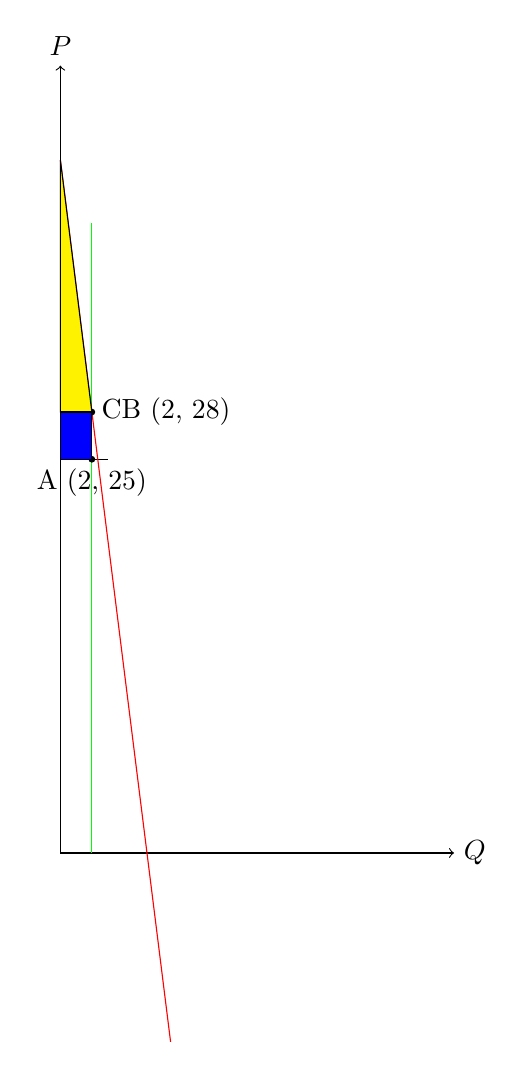
\begin{tikzpicture}
          \draw [->] (0,0) -- (5,0)node[right] {$Q$};
          \draw [->] (0,0) -- (0,10)node[above] {$P$};
          \draw [-, scale = 0.2, color=green] (2,0) -- (2,40);
          \draw [-, scale = 0.2, color=black] (0,25) -- (3,25);
          \draw[scale = 0.2, domain=0:7, smooth, variable=\x, color=red]
          plot ({\x}, {44 - 8 * \x});
          \filldraw[scale = 0.2, color=black] (2, 28)
          circle (5pt) node[anchor=west]{CB (2, 28)};
          \filldraw[scale = 0.2, color=black] (2, 25)
          circle (5pt) node[anchor=north]{A (2, 25)};

          \filldraw[fill=yellow, scale = 0.2] (0,28) -- (2,28) -- (0, 44) -- cycle;
          \filldraw[fill=blue, scale = 0.2] (0,28) -- (2,28) -- (2, 25) -- (0, 25) -- cycle;
        \end{tikzpicture}



    tại mức giá này CS = (44 - 28) * 2 / 2 + 2 * (28 - 25) = 16 + 6 = 22 và PS vẫn không xác định

\end{enumerate}

\section{Cung và cầu của hàng hóa X có phương trình như sau:}

$Q_D = 150 - 5P$ và $Q_S = 5P - 10$

\begin{enumerate}[a.]
  \item Tính giá và lượng cân bằng trên thị trường.
  
  $150 - 5P = 5P - 10$\\
  $10P = 160 \Rightarrow P = 16 \Rightarrow Q = 70$

  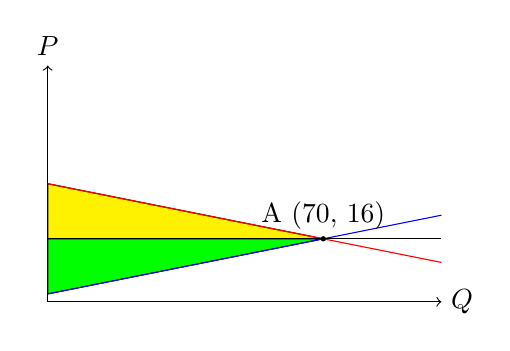
\begin{tikzpicture}
    \draw [->] (0,0) -- (5,0)node[right] {$Q$};
    \draw [->] (0,0) -- (0,3)node[above] {$P$};

    \filldraw[fill=yellow, scale = 0.05] (0,16) -- (70,16) -- (0, 30) -- cycle;
    \filldraw[fill=green, scale = 0.05] (0,16) -- (70,16) -- (0, 2) -- cycle;

    \draw[scale = 0.05, domain=0:100, smooth, variable=\x, color=red]
    plot ({\x}, {30 - \x / 5});
    \draw[scale = 0.05, domain=0:100, smooth, variable=\x, color=blue]
    plot ({\x}, {\x / 5 + 2});
    
    \filldraw[scale = 0.05, color=black] (70, 16)
    circle (15pt) node[anchor=south]{A (70, 16)};

    \draw [-, scale = 0.05, color=black] (0,16) -- (100,16);
   
    
 

  \end{tikzpicture}

  \item Nếu giá bán trên thị trường là P = 18 thì điều gì xảy ra trên thị trường? 
  
   hiện tượng dư cung, dư thừa hàng hóa xảy ra
  
  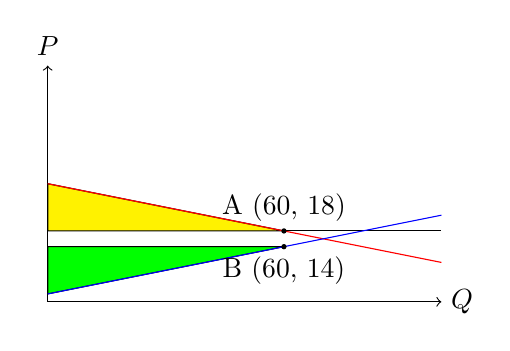
\begin{tikzpicture}
    \draw [->] (0,0) -- (5,0)node[right] {$Q$};
    \draw [->] (0,0) -- (0,3)node[above] {$P$};

    \draw [-, scale = 0.05, color=black] (0,18) -- (100,18);
    \filldraw[fill=yellow, scale = 0.05] (0,18) -- (60,18) -- (0, 30) -- cycle;
    \filldraw[fill=green, scale = 0.05] (0,14) -- (60,14) -- (0, 2) -- cycle;

    \draw[scale = 0.05, domain=0:100, smooth, variable=\x, color=red]
    plot ({\x}, {30 - \x / 5});
    \draw[scale = 0.05, domain=0:100, smooth, variable=\x, color=blue]
    plot ({\x}, {\x / 5 + 2});
    
    \filldraw[scale = 0.05, color=black] (60, 14)
    circle (15pt) node[anchor=north]{B (60, 14)};
    \filldraw[scale = 0.05, color=black] (60, 18)
    circle (15pt) node[anchor=south]{A (60, 18)};

   
  \end{tikzpicture}

  \item So sánh thặng dư sản xuất và thặng dư tiêu dùng tại trạng thái cân bằng và khi P = 18
  
   tại trạng thái cân bằng,\\
    CS = (30 - 16) * 70 / 2 = 14 * 35 \\
    PS = (16 - 2) * 70 / 2 = 14 * 35 \\
  tại P = 18 \\
  CS = (30 - 18) * 60 / 2 = 12 * 30 \\
  PS = (14 - 2) * 60 / 2 = 12 * 30 \\
  

\end{enumerate}

\section{Hàm cầu và hàm cung của trứng gà như sau:}

$P_D = 10 - Q$ và $ P_S = Q - 4$ \\
(P tình bằng nghìn đồng/1 quả, Q tính bằng triệu quả)


\begin{enumerate}[a.]
  \item .Tính giá và sản lượng cân bằng trên thị trường. Tính hệ số co giãn của cung và cầu tại
        mức giá cân bằng.

        chúng ta có $P_D = 10 - Q$ và $ P_S = Q - 4$ \\
        $10 -Q = Q - 4 \Rightarrow Q = 7, P = 3 $ là giá và sản lượng cân bằng

        chúng ta có công thức tính hệ số co giãn của cầu như sau
        \[ E_{DP} = \frac{\%\Delta Q_D}{\%\Delta P} =
          \frac{\Delta Q_D}{\Delta P} \times \frac{P}{Q_D} = Q_D' \times \frac{P}{Q_D} \]

        $Q_D' = ( 10 - P)' = -1$ \\
        vậy $E_{DP} = (-1) * 3 / 7 = -0.428 $

        chúng ta có công thức tính hệ số co giãn của cung như sau
        \[ E_{SP} = \frac{\%\Delta Q_S}{\%\Delta P} =
          \frac{\Delta Q_S}{\Delta P} \times \frac{P}{Q_S} = Q_S' \times \frac{P}{Q_S} \]

        $Q_S' = ( 4 + P)' = 1$ \\
        vậy $E_{SP} = (1) * 3 / 7 = 0.428 $

  \item Tính thặng dư sản xuất và thặng dư tiêu dùng tại mức giá cân bằng.
        chúng ta cần vẽ hình ra để dễ nhìn hơn

        CS = (10 - 3) * (7 - 0) / 2 = 49 / 2\\
        PS = ( 3 - (-4))  * (7 - 0) / 2 = 49 / 2\\

        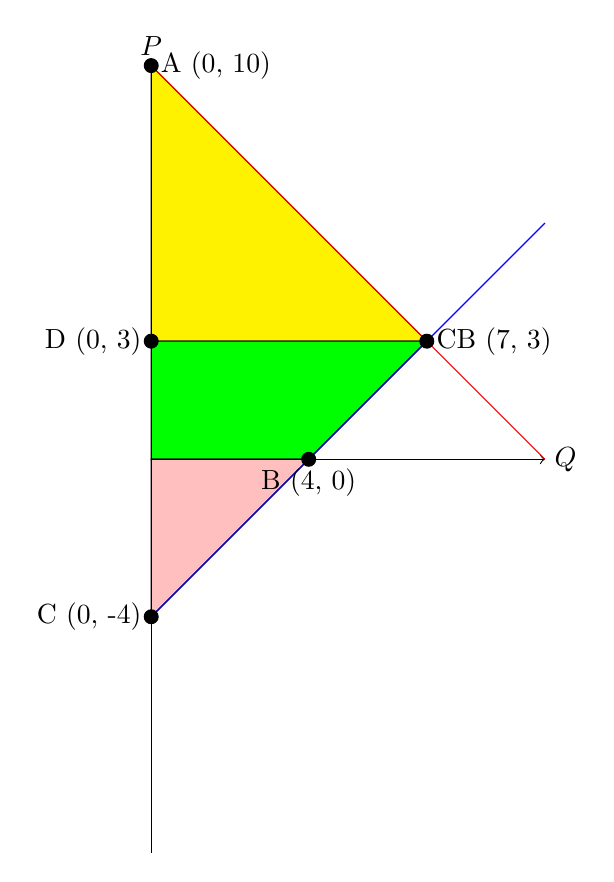
\begin{tikzpicture}
          \draw [->] (0,0) -- (5,0)node[right] {$Q$};
          \draw [->] (0,-5) -- (0,5)node[above] {$P$};

          \filldraw[fill=yellow, scale = 0.5] (0,3) -- (7,3) -- (0, 10) -- cycle;
          \filldraw[fill=green, scale = 0.5] (0,3) -- (7,3) -- (4, 0) -- (0, 0) -- cycle;
          \filldraw[fill=pink, scale = 0.5] (0,-4) --  (4, 0) -- (0, 0) -- cycle;

          \draw[scale = 0.5, domain=0:10, smooth, variable=\x, color=red]
          plot ({\x}, {10 - \x});
          \draw[scale = 0.5, domain=0:10, smooth, variable=\x, color=blue]
          plot ({\x}, {\x - 4});

          \filldraw[scale = 0.5, color=black] (7, 3)
          circle (5pt) node[anchor=west]{CB (7, 3)};
          \filldraw[scale = 0.5, color=black] (0, 10)
          circle (5pt) node[anchor=west]{A (0, 10)};
          \filldraw[scale = 0.5, color=black] (4, 0)
          circle (5pt) node[anchor=north]{B (4, 0)};

          \filldraw[scale = 0.5, color=black] (0, -4)
          circle (5pt) node[anchor=east]{C (0, -4)};

          \filldraw[scale = 0.5, color=black] (0, 3)
          circle (5pt) node[anchor=east]{D (0, 3)};

          %\draw [-, scale = 0.05, color=black] (0,16) -- (100,16);




        \end{tikzpicture}

  \item Khi giá bán trên thị trường P= 2 nghìn đồng/quả. Thặng dư sản xuất và thặng dư tiêu
        dùng thay đổi như thế nào so với trước?

        CS = (10 - 4) * (6 - 0) / 2 = 18\\
        PS = ( 2 - (-4))  * (6 - 0) / 2 = 18\\

        kết luận: thặng du sản xuất PS giảm, thặng dư tiêu dùng CS giảm

        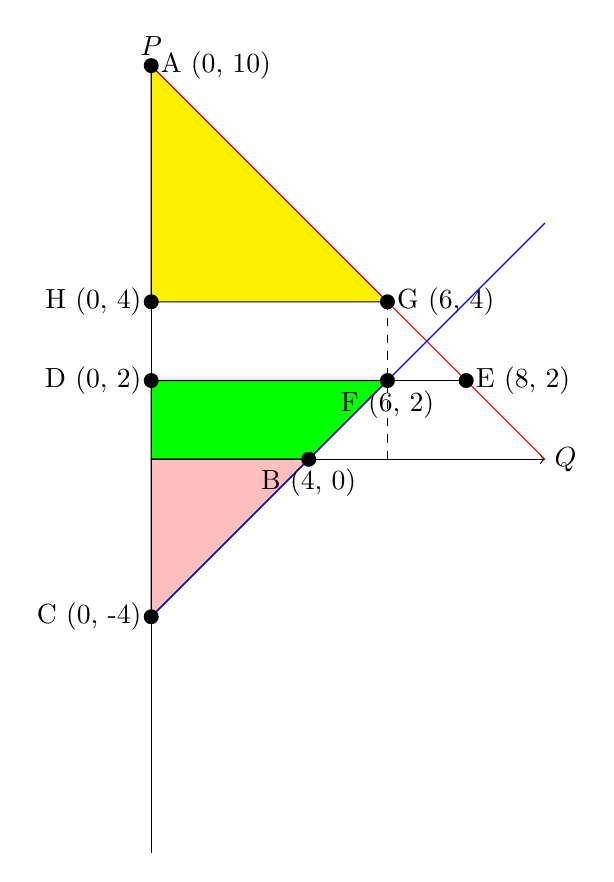
\begin{tikzpicture}
          \draw [->] (0,0) -- (5,0)node[right] {$Q$};
          \draw [->] (0,-5) -- (0,5)node[above] {$P$};

          \filldraw[fill=yellow, scale = 0.5] (0,4) -- (6,4) -- (0, 10) -- cycle;
          \filldraw[fill=green, scale = 0.5] (0,2) -- (6,2) -- (4, 0) -- (0, 0) -- cycle;
          \filldraw[fill=pink, scale = 0.5] (0,-4) --  (4, 0) -- (0, 0) -- cycle;
          %\filldraw[fill=olive, scale = 0.5] (0,3) -- (7,3) -- (8, 2) -- (0, 2) -- cycle;

          \draw[scale = 0.5, domain=0:10, smooth, variable=\x, color=red]
          plot ({\x}, {10 - \x});
          \draw[scale = 0.5, domain=0:10, smooth, variable=\x, color=blue]
          plot ({\x}, {\x - 4});
          \draw [dashed, scale = 0.5] (6,0) -- (6,4);
          

          \filldraw[scale = 0.5, color=black] (8, 2)
          circle (5pt) node[anchor=west]{E (8, 2)};
          \filldraw[scale = 0.5, color=black] (0, 10)
          circle (5pt) node[anchor=west]{A (0, 10)};
          \filldraw[scale = 0.5, color=black] (4, 0)
          circle (5pt) node[anchor=north]{B (4, 0)};

          \filldraw[scale = 0.5, color=black] (0, -4)
          circle (5pt) node[anchor=east]{C (0, -4)};

          \filldraw[scale = 0.5, color=black] (0, 2)
          circle (5pt) node[anchor=east]{D (0, 2)};
          \filldraw[scale = 0.5, color=black] (6, 2)
          circle (5pt) node[anchor=north]{F (6, 2)};
          \filldraw[scale = 0.5, color=black] (6, 4)
          circle (5pt) node[anchor=west]{G (6, 4)};
          \filldraw[scale = 0.5, color=black] (0, 4)
          circle (5pt) node[anchor=east]{H (0, 4)};

          \draw [-, scale = 0.5, color=black] (0,2) -- (8, 2);

        \end{tikzpicture}

\end{enumerate}
\chapter{CHÍNH SÁCH CỦA
  CHÍNH PHỦ}

\section{ Sản phẩm X có hàm cung và hàm cầu là:}
$Q_S = P - 20 $  $ Q_D = 120 - P$ \\
(P tính bằng nghìn đồng/tấn, Q tính bằng triệu tấn)

\begin{enumerate}[a.]
    \item Xác định giá và sản lượng cân bằng trên thị trường.

          $Q_S = P - 20 = Q_D = 120 - P$
          $\Rightarrow 2P = 140 \Rightarrow P = 70, Q = 50$

    \item Chính phủ áp đặt mức giá trần $P_C= 50$ nghìn đồng/tấn thì điều gì xảy ra trên thị trường?
          Tại sao? Tính CS, PS tại mức giá trần này.



          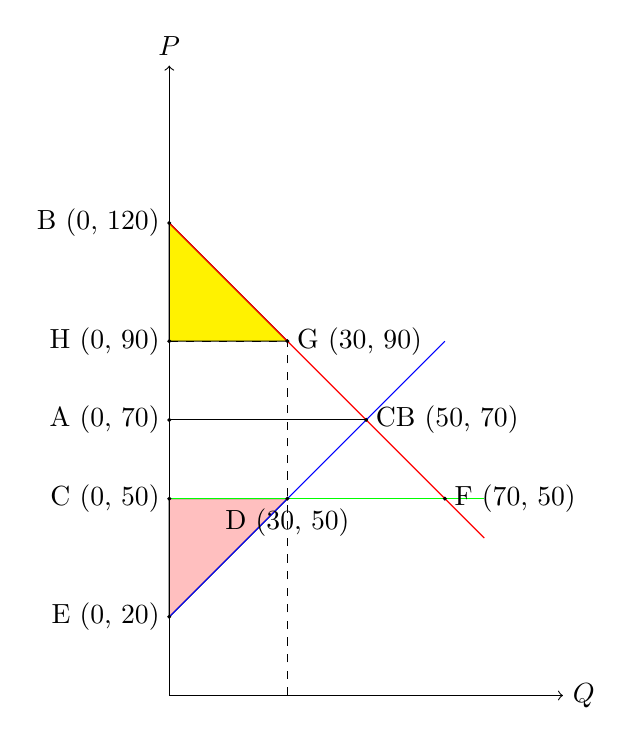
\begin{tikzpicture}
              \draw [->] (0,0) -- (5,0)node[right] {$Q$};
              \draw [->] (0,0) -- (0,8)node[above] {$P$};

              \filldraw[fill=yellow, scale = 0.05] (0,90) -- (30,90) -- (0, 120) -- cycle;
              %\filldraw[fill=green, scale = 0.5] (0,3) -- (7,3) -- (4, 0) -- (0, 0) -- cycle;
              \filldraw[fill=pink, scale = 0.05] (0,50) --  (30, 50) -- (0, 20) -- cycle;

              \draw[scale = 0.05, domain=0:80, smooth, variable=\x, color=red]
              plot ({\x}, {120 - \x});
              \draw[scale = 0.05, domain=0:70, smooth, variable=\x, color=blue]
              plot ({\x}, {\x + 20});

              \draw [-, scale = 0.05, color=green] (0,50) -- (80,50);
              \draw [-, scale = 0.05, color=black] (0,70) -- (50,70);
              \draw [dashed, scale = 0.05, color=black] (30,0) -- (30,90);
              \draw [dashed, scale = 0.05, color=black] (0,90) -- (30,90);

              \filldraw[scale = 0.05, color=black] (50, 70)          circle (10pt) node[anchor=west]{CB (50, 70)};
              \filldraw[scale = 0.05, color=black] (0, 70)          circle (10pt) node[anchor=east]{A (0, 70)};
              \filldraw[scale = 0.05, color=black] (0, 120)          circle (10pt) node[anchor=east]{B (0, 120)};

              \filldraw[scale = 0.05, color=black] (0, 50)          circle (10pt) node[anchor=east]{C (0, 50)};

              \filldraw[scale = 0.05, color=black] (30, 50)          circle (10pt) node[anchor=north]{D (30, 50)};

              \filldraw[scale = 0.05, color=black] (70, 50)          circle (10pt) node[anchor=west]{F (70, 50)};

              \filldraw[scale = 0.05, color=black] (0, 20)          circle (10pt) node[anchor=east]{E (0, 20)};
              \filldraw[scale = 0.05, color=black] (30, 90)          circle (10pt) node[anchor=west]{G (30, 90)};
              \filldraw[scale = 0.05, color=black] (0, 90)          circle (10pt) node[anchor=east]{H (0, 90)};

          \end{tikzpicture}

          tình trạng hiện tại là dư cầu \\
          CS = diện tích BHG = (120 - 90) * 30 / 2 = 450 , \\
          PS = diện tích CDE = (50 - 20) * 30 / 2 = 450


    \item Nếu chính phủ áp đặt giá sàn $P_f = 80$ nghìn đồng/tấn thì điều gì xảy ra trên thị trường?
          Tại sao? Tính CS, PS tại mức giá sàn này.
          Để cho mức giá sàn có hiệu lực thì nhà nước phải làm gì? Số tiền chính phủ phải chi ra
          là bao nhiêu?

          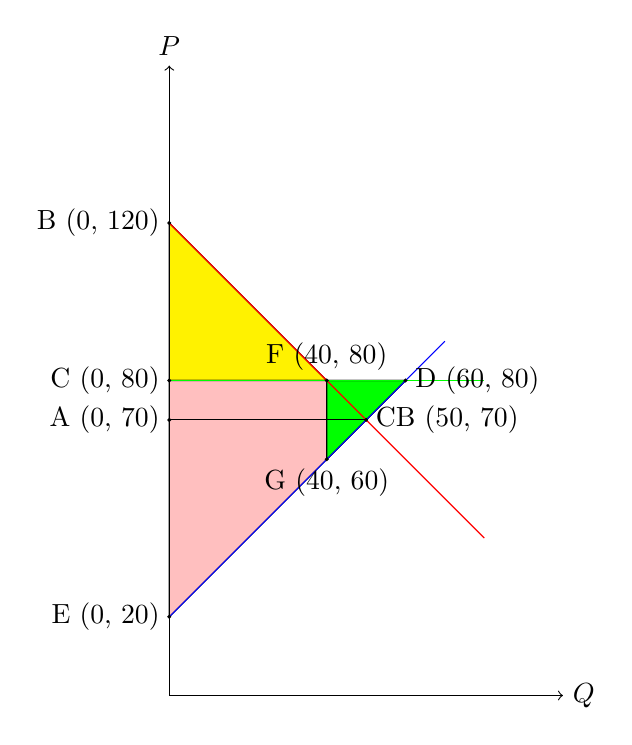
\begin{tikzpicture}
              \draw [->] (0,0) -- (5,0)node[right] {$Q$};
              \draw [->] (0,0) -- (0,8)node[above] {$P$};

              \filldraw[fill=yellow, scale = 0.05] (0,80) -- (40,80) -- (0, 120) -- cycle;
              \filldraw[fill=pink, scale = 0.05] (0,80) --  (60, 80) -- (0, 20) -- cycle;
              \filldraw[fill=green, scale = 0.05] (40,80) -- (60, 80) -- (40, 60) -- cycle;

              \draw[scale = 0.05, domain=0:80, smooth, variable=\x, color=red]
              plot ({\x}, {120 - \x});
              \draw[scale = 0.05, domain=0:70, smooth, variable=\x, color=blue]
              plot ({\x}, {\x + 20});

              \draw [-, scale = 0.05, color=green] (0,80) -- (80,80);
              \draw [-, scale = 0.05, color=black] (0,70) -- (50,70);

              \filldraw[scale = 0.05, color=black] (50, 70)          circle (10pt) node[anchor=west]{CB (50, 70)};
              \filldraw[scale = 0.05, color=black] (0, 70)          circle (10pt) node[anchor=east]{A (0, 70)};
              \filldraw[scale = 0.05, color=black] (0, 120)          circle (10pt) node[anchor=east]{B (0, 120)};

              \filldraw[scale = 0.05, color=black] (0, 80)          circle (10pt) node[anchor=east]{C (0, 80)};

              \filldraw[scale = 0.05, color=black] (60, 80)          circle (10pt) node[anchor=west]{D (60, 80)};

              \filldraw[scale = 0.05, color=black] (40, 80)          circle (10pt) node[anchor=south]{F (40, 80)};

              \filldraw[scale = 0.05, color=black] (0, 20)          circle (10pt) node[anchor=east]{E (0, 20)};

              \filldraw[scale = 0.05, color=black] (40, 60)          circle (10pt) node[anchor=north]{G (40, 60)};

          \end{tikzpicture}

          tình trạng hiện tại là dư cung \\
          CS = diện tích BCF = (120 - 80) * 40 / 2 = 800 , \\
          PS = diện tích CDE = (80 - 20) * 60 / 2 = 1800 \\
          Để cho mức giá sàn có hiệu lực thì nhà nước phải làm gì? Số tiền chính phủ phải chi ra
          là bao nhiêu? \\
          để áp đặt mức giá này thì chính phủ cần thu mua số lượng hàng dư thừa
          lượng tiền bỏ ra là diện tích FGD = (60 - 40) * (80 - 60) / 2 = 200

\end{enumerate}

\section{ Thị trường thịt gà có phương trình hàm cung và cầu như sau:}
$Q_S = 2,5P - 12,5$  $Q_D = 100 - 2P$ \\
(P tính bằng nghìn đồng/kg, Q tính bằng triệu kg)

\begin{enumerate}[a.]
  \item Xác định giá và sản lượng cân bằng trên thị trường.

        $Q_S = 2.5P - 12.5 = Q_D = 100 -   2P$
        $\Rightarrow 4.5P = 112.5 \Rightarrow P = 25, Q = 50$

  \item Nếu chính phủ đánh thuế 1,8 nghìn đồng/1kg vào người bán thì giá mới sẽ là bao nhiêu?
        Giá người bán, người mua phải chịu là bao nhiêu? Thuế mà người mua và người bán phải
        nộp là bao nhiêu?

        ta lưu ý tại hình 6.5 slide 5: Đường cung dịch chuyển lên trên 1 khoảng đúng  bằng mức thuế t

        $Q_S = 2.5P - 12.5 \Rightarrow P = Q_S / 2.5 + 5$ \\
        $P = Q_S / 2.5 + 5 + 1.8 = Q_S / 2.5 + 6.8$\\
        điểm cân bằng mới sẽ tính như sau \\
        $P = Q_S / 2.5 + 6.8 \Rightarrow Q_S = 2.5P - 17 = Q_D = 100 - 2P$\\
        $4.5P = 117 \Rightarrow P = 26, Q = 48$ giá mới là 26


        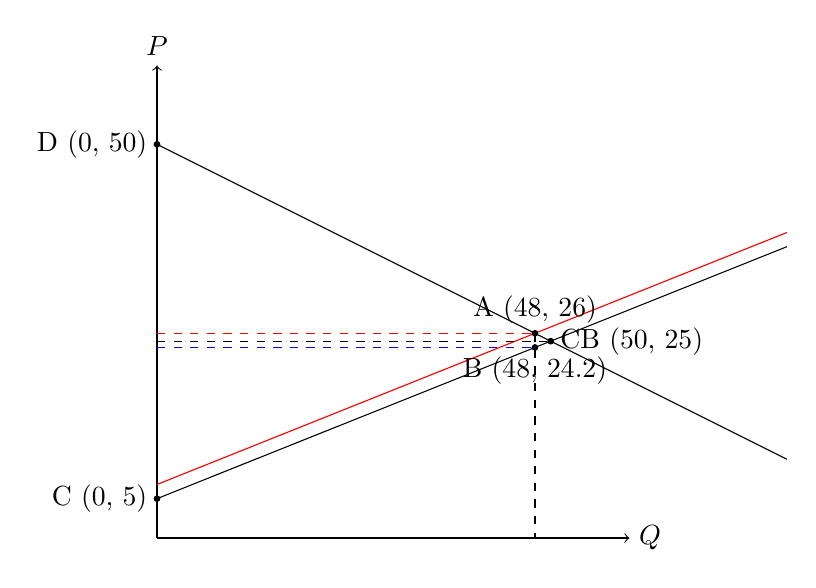
\begin{tikzpicture}
          \draw [->] (0,0) -- (6,0)node[right] {$Q$};
          \draw [->] (0,0) -- (0,6)node[above] {$P$};

          \draw[scale = 0.1, domain=0:80, smooth, variable=\x, color=black]
          plot ({\x}, {50 - \x / 2});
          \draw[scale = 0.1, domain=0:80, smooth, variable=\x, color=black]
          plot ({\x}, {\x / 2.5 + 5});
          \draw[scale = 0.1, domain=0:80, smooth, variable=\x, color=red]
          plot ({\x}, {\x / 2.5 + 6.8});


          \draw [dashed, scale = 0.1, color=black] (0,25) -- (50,25);
          \draw [dashed, scale = 0.1, color=black] (48, 26) -- (48, 0);
          \draw [dashed, scale = 0.1, color=red] (0, 26) -- (48, 26);
          \draw [dashed, scale = 0.1, color=blue] (0, 24.2) -- (48, 24.2);


          \filldraw[scale = 0.1, color=black] (50, 25) circle (10pt) node[anchor=west]{CB (50, 25)};
          \filldraw[scale = 0.1, color=black] (48, 26)  circle (10pt) node[anchor=south]{A (48, 26)};
          \filldraw[scale = 0.1, color=black] (48, 24.2)  circle (10pt) node[anchor=north]{B (48, 24.2)};
          \filldraw[scale = 0.1, color=black] (0, 5)  circle (10pt) node[anchor=east]{C (0, 5)};
          \filldraw[scale = 0.1, color=black] (0, 50)  circle (10pt) node[anchor=east]{D (0, 50)};          

        \end{tikzpicture}

        Giá người bán chịu là giao của đường cung và đường song song với trục tung và đi qua điểm cân bằng mới tại đó Q = 48 do đó P = 24.2,\\
        giá người người mua phải chịu là giá tại điểm cân bằng mới P = 26 \\
        Thuế mà người mua là khoảng cách giữa giá mua và giá cân bằng trước thuế = 26 - 25 = 1\\
        thuế người bán phải nộp là khoảng cách giữa giá thực bán và giá cân bằng trước thuế = 25 - 24.2 = 0.8

  \item Vẽ đồ thị minh họa tác động của thuế ở câu b? Tính CS, PS, TS và phần mất không (DWL)
        của việc đánh thuế này?

        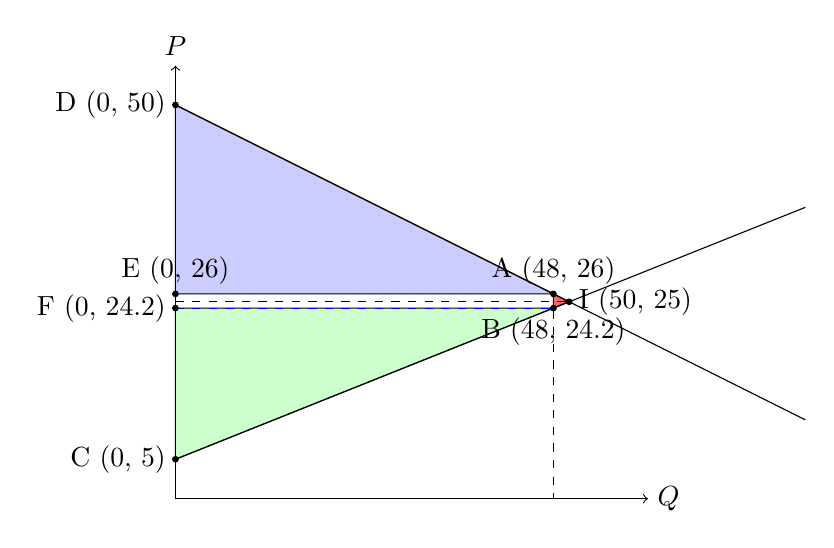
\begin{tikzpicture}
          \draw [->] (0,0) -- (6,0)node[right] {$Q$};
          \draw [->] (0,0) -- (0,5.5)node[above] {$P$};

          \filldraw[fill=blue!20, scale = 0.1] (0,50) -- (48,26) -- (0, 26) -- cycle;
          \filldraw[fill=green!20, scale = 0.1] (0,24.2) -- (48,24.2) -- (0, 5) -- cycle;
          \filldraw[fill=red!60, scale = 0.1] (50,25) -- (48,26) -- (48, 24.2) -- cycle;

          \draw[scale = 0.1, domain=0:80, smooth, variable=\x, color=black]
          plot ({\x}, {50 - \x / 2});
          \draw[scale = 0.1, domain=0:80, smooth, variable=\x, color=black]
          plot ({\x}, {\x / 2.5 + 5});
          %\draw[scale = 0.1, domain=0:80, smooth, variable=\x, color=red] plot ({\x}, {\x / 2.5 + 6.8});


          \draw [dashed, scale = 0.1, color=black] (0,25) -- (50,25);
          \draw [dashed, scale = 0.1, color=black] (48, 26) -- (48, 0);
          \draw [dashed, scale = 0.1, color=red] (0, 26) -- (48, 26);
          \draw [dashed, scale = 0.1, color=blue] (0, 24.2) -- (48, 24.2);


          \filldraw[scale = 0.1, color=black] (50, 25) circle (10pt) node[anchor=west]{I (50, 25)};
          \filldraw[scale = 0.1, color=black] (48, 26)  circle (10pt) node[anchor=south]{A (48, 26)};
          \filldraw[scale = 0.1, color=black] (48, 24.2)  circle (10pt) node[anchor=north]{B (48, 24.2)};
          
          \filldraw[scale = 0.1, color=black] (0, 5)  circle (10pt) node[anchor=east]{C (0, 5)};
          \filldraw[scale = 0.1, color=black] (0, 50)  circle (10pt) node[anchor=east]{D (0, 50)};
          
          \filldraw[scale = 0.1, color=black] (0, 26)  circle (10pt) node[anchor=south]{E (0, 26)};
          \filldraw[scale = 0.1, color=black] (0, 24.2)  circle (10pt) node[anchor=east]{F (0, 24.2)};
          

        \end{tikzpicture}

        CS  = diện tích ADE = (50 - 26) * 48 / 2 = 24 * 24\\
        PS  = diện tích BFC = (24.2 - 5) * 48 / 2\\
        DWL = diện tích ABI = (26 - 24.2) * (50 - 48) / 2\\
        TS = CS + PS  \\

  \item Nếu chính phủ trợ cấp cho người bán là 1,8 nghìn đồng/1kg, giá mới sẽ là bao nhiêu?
        Mỗi bên được hưởng bao nhiêu trợ cấp? Số tiền trợ cấp mà chính phủ phải chi ra là bao
        nhiêu?

        khi đó $P_S - P_D = 1.8$ do trợ cấp nên $P_S$ lớn hơn $P_D$\\
        ta có $Q_S = 2,5P - 12,5$  $Q_D = 100 - 2P$ \\
        hay $Q / 2.5 + 5 -( 50 - Q/ 2) = 1.8$ \\
        $Q / 2.5 + Q / 2 = 50 - 5 + 1.8 = 46.8  $ \\
        nhân 5 cho 2 vế ta có \\
        $ 2Q + 2.5 Q =  234 \Rightarrow Q = 52 \Rightarrow P_S = 52/2.5 + 5 = 25.8, P_D = 50 - 52 = 24$


        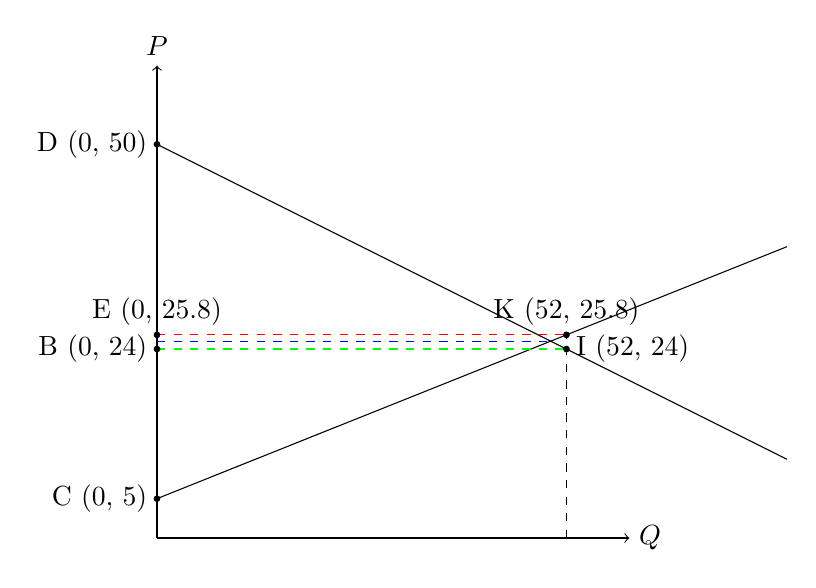
\begin{tikzpicture}
          \draw [->] (0,0) -- (6,0)node[right] {$Q$};
          \draw [->] (0,0) -- (0,6)node[above] {$P$};

          %\filldraw[fill=blue!20, scale = 0.1] (0,50) -- (52,24) -- (0, 24) -- cycle;
          %\filldraw[fill=green!20, scale = 0.1] (0,3.2) -- (52,24) -- (0, 24) -- cycle;

          \draw[scale = 0.1, domain=0:80, smooth, variable=\x, color=black]
          plot ({\x}, {50 - \x / 2});
          \draw[scale = 0.1, domain=0:80, smooth, variable=\x, color=black]
          plot ({\x}, {\x / 2.5 + 5});


          \draw [dashed, scale = 0.1, color=black] (52,0) -- (52, 25.8);
          \draw [dashed, scale = 0.1, color=green] (0, 24) -- (52, 24);
          \draw [dashed, scale = 0.1, color=red] (0, 25.8) -- (52, 25.8);
          \draw [dashed, scale = 0.1, color=blue] (0, 25) -- (50, 25);


          \filldraw[scale = 0.1, color=black] (52, 24) circle (10pt) node[anchor=west]{I (52, 24)};
          \filldraw[scale = 0.1, color=black] (52, 25.8) circle (10pt) node[anchor=south]{K (52, 25.8)};
          %\filldraw[scale = 0.1, color=black] (0, 3.2)  circle (10pt) node[anchor=west]{A (0, 3.2)};
          \filldraw[scale = 0.1, color=black] (0, 24)  circle (10pt) node[anchor=east]{B (0, 24)};
          \filldraw[scale = 0.1, color=black] (0, 5)  circle (10pt) node[anchor=east]{C (0, 5)};
          \filldraw[scale = 0.1, color=black] (0, 50)  circle (10pt) node[anchor=east]{D (0, 50)};          

          \filldraw[scale = 0.1, color=black] (0, 25.8)  circle (10pt) node[anchor=south]{E (0, 25.8)};          

        \end{tikzpicture}

        Mỗi bên được hưởng bao nhiêu trợ cấp? Số tiền trợ cấp mà chính phủ phải chi ra là bao
        nhiêu? \\
        khoản trợ cấp của bên mua là chênh lệch giữa giá cân bằng và giá sau trợ cấp nhân với lượng cầu tại giá trợ cấp tức là : \\
        $(25 - 24) * 52$ \\
        khoản trợ cấp của bên bán là chênh lệch giữa giá cân bằng và giá sau trợ cấp nhân với lượng cung tại giá trợ cấp tức là : \\
        $(25.8 - 25) * 52$ \\
        số tiền trợ cấp của chính phủ là tích của mức trợ cấp nhân với sản lượng \\
        $1.8 * 52$
        
\end{enumerate}


\section{Thị trường mỳ tôm có phương trình }
đường cung $Q_S = 30 + 2P$ và phương trình
đường cầu $Q_D = 180 - 3P$ (P tính theo nghìn đồng/kg, Q tính theo triệu kg).: \\
(P tính bằng nghìn đồng/kg, Q tính bằng triệu kg) \\

\begin{enumerate}[a.]
  \item Tìm giá và lượng cân bằng trên thị trường? \\
        $Q_S = 30 + 2P = Q_D = 180 - 3P \Rightarrow 5P = 150 \Rightarrow P = 30, Q = 90$
  \item Giả sử chính phủ đánh thuế 10 nghìn đồng trên mỗi kg sản phẩm mà người tiêu dùng
        mua. Xác định giá và lượng cân bằng sau thuế? Tính gánh nặng thuế đối với người tiêu
        dùng và người sản xuất, số tiền thuế mà chính phủ thu được là bao nhiêu? \\
        theo 6.2.2 thì khi thuế đánh vào người mua; "Đường cầu dịch
        chuyển xuống dưới  1 khoảng đúng bằng  mức thuế t" \\
        ta viết phương trình đường cầu cũ:  \\
        $Q_D = 180 - 3P$\\
        phương trình cầu sau thuế là \\
        $P + 10 = 60 - Q_D / 3$ với ý nghĩa là với lương hàng hóa nhu cũ thì cần thêm 10 đồng mới mua được \\
        $P = 60 - Q_D / 3 - 10 = 50 - Q_D / 3 \Rightarrow Q_D = 150 -3P$\\
        điểm cân bằng mới tính như sau\\
        $150 - 3P = 30 + 2P \Rightarrow 5P = 120 \Rightarrow P = 24, Q = 78$

        ta sẽ vẽ đồ thị để dễ nhìn hơn \\
        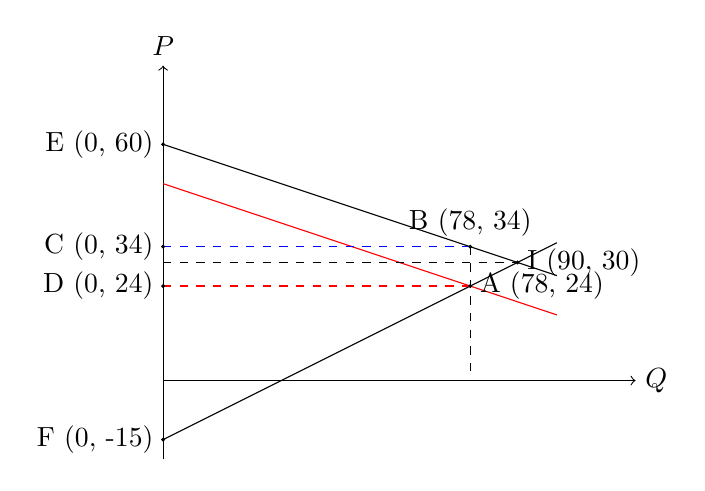
\begin{tikzpicture}
          \draw [->] (0,0) -- (6,0)node[right] {$Q$};
          \draw [->] (0,-1) -- (0,4)node[above] {$P$};

          \draw[scale = 0.05, domain=0:100, smooth, variable=\x, color=black]
          plot ({\x}, {\x / 2 - 15});
          \draw[scale = 0.05, domain=0:100, smooth, variable=\x, color=black]
          plot ({\x}, {60 - \x / 3 });
          \draw[scale = 0.05, domain=0:100, smooth, variable=\x, color=red]
          plot ({\x}, {50 - \x / 3});


          \draw [dashed, scale = 0.05, color=black] (0,30) -- (90,30);
          \draw [dashed, scale = 0.05, color=black] (78, 34) -- (78, 0);
          \draw [dashed, scale = 0.05, color=red] (0, 24) -- (78, 24);
          \draw [dashed, scale = 0.05, color=blue] (0, 34) -- (78, 34);


          \filldraw[scale = 0.05, color=black] (90, 30) circle (10pt) node[anchor=west]{I (90, 30)};
          \filldraw[scale = 0.05, color=black] (78, 24)  circle (10pt) node[anchor=west]{A (78, 24)};
          \filldraw[scale = 0.05, color=black] (78, 34)  circle (10pt) node[anchor=south]{B (78, 34)};
          \filldraw[scale = 0.05, color=black] (0, 34)  circle (10pt) node[anchor=east]{C (0, 34)};
          \filldraw[scale = 0.05, color=black] (0, 24)  circle (10pt) node[anchor=east]{D (0, 24)};
          \filldraw[scale = 0.05, color=black] (0, 60)  circle (10pt) node[anchor=east]{E (0, 60)};
          \filldraw[scale = 0.05, color=black] (0, -15)  circle (10pt) node[anchor=east]{F (0, -15)};
        \end{tikzpicture}

        Xác định giá và lượng cân bằng sau thuế? $P = 24, Q = 78$\\
        Tính gánh nặng thuế đối với người tiêu dùng và người sản xuất, số tiền thuế mà chính phủ thu được là bao nhiêu?\\
        với người tiêu dùng = 34 - 30 \\
        với người sản xuất = 30 - 24\\
        số tiền thuế = $S_{CBAD} = 78 * (34 - 24)$

  \item  Với mức thuế ở câu b, tính CS, PS, phần mất không do thuế gây ra là bao nhiêu?

        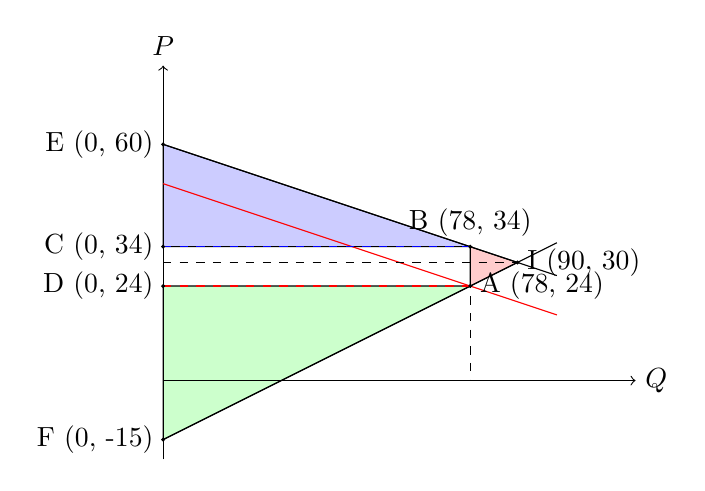
\begin{tikzpicture}


          \filldraw[fill=blue!20, scale = 0.05] (0,60) -- (78,34) -- (0, 34) -- cycle;
          \filldraw[fill=red!20, scale = 0.05] (78, 34) -- (90, 30) -- (78, 24) -- cycle;
          \filldraw[fill=green!20, scale = 0.05] (0 ,24) -- (78,24) -- (0, -15) -- cycle;

          \draw [->] (0,0) -- (6,0)node[right] {$Q$};
          \draw [->] (0,-1) -- (0,4)node[above] {$P$};

          \draw[scale = 0.05, domain=0:100, smooth, variable=\x, color=black]
          plot ({\x}, {\x / 2 - 15});
          \draw[scale = 0.05, domain=0:100, smooth, variable=\x, color=black]
          plot ({\x}, {60 - \x / 3 });
          \draw[scale = 0.05, domain=0:100, smooth, variable=\x, color=red]
          plot ({\x}, {50 - \x / 3});

          \draw [dashed, scale = 0.05, color=black] (0,30) -- (90,30);
          \draw [dashed, scale = 0.05, color=black] (78, 34) -- (78, 0);
          \draw [dashed, scale = 0.05, color=red] (0, 24) -- (78, 24);
          \draw [dashed, scale = 0.05, color=blue] (0, 34) -- (78, 34);


          \filldraw[scale = 0.05, color=black] (90, 30) circle (10pt) node[anchor=west]{I (90, 30)};
          \filldraw[scale = 0.05, color=black] (78, 24)  circle (10pt) node[anchor=west]{A (78, 24)};
          \filldraw[scale = 0.05, color=black] (78, 34)  circle (10pt) node[anchor=south]{B (78, 34)};
          \filldraw[scale = 0.05, color=black] (0, 34)  circle (10pt) node[anchor=east]{C (0, 34)};
          \filldraw[scale = 0.05, color=black] (0, 24)  circle (10pt) node[anchor=east]{D (0, 24)};
          \filldraw[scale = 0.05, color=black] (0, 60)  circle (10pt) node[anchor=east]{E (0, 60)};
          \filldraw[scale = 0.05, color=black] (0, -15)  circle (10pt) node[anchor=east]{F (0, -15)};
        \end{tikzpicture}

        CS = diện tích CEB = (60 - 34) * 78 / 2 \\
        PS = diện tích DFA = (24 - (-15)) * 78 / 2\\
        DWL = diện tích BAI = (34 - 24) * (90 - 78) / 2\\
        mọi người có thể ngạc nhiên về PS, tại sao lại có số -15, trong kinh tế, bán hàng giá âm chưa chắc đã là lỗ mà bán hàng giá dương chưa chắc đã là lãi

  \item Nếu chính phủ trợ cấp 10 nghìn đồng/kg mỳ tôm mà người tiêu dùng mua. Giá và sản
        lượng sẽ thay đổi như thế nào? Mỗi bên được hưởng bao nhiêu trợ cấp?

        khi nhận trợ cấp thì $P_S$ sẽ lớn hơn $P_D$ và $P_S - P_D = 10$ \\ 
        ta có các phương trình như sau\\
        $Q_S = 30 + 2P \Rightarrow P = Q_S / 2 - 15$ \\
        $Q_D = 180 - 3P \Rightarrow P = 60 - Q_D / 3$ \\
        $Q/ 2 - 15 - (60 - Q/ 3) = 10 \Rightarrow Q / 2 + Q / 3 = 15 + 60 + 10 = 85$ \\
        nhân 6 cho 2 vế \\
        $3 Q + 2 Q = 85 * 6 \Rightarrow Q = 102, P_S = 36, P_D = 26$

        

        ta sẽ vẽ đồ thị để dễ nhìn hơn \\
        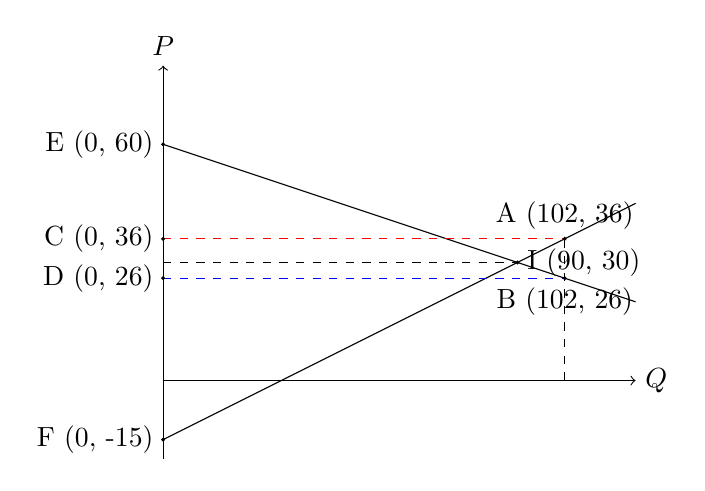
\begin{tikzpicture}
          \draw [->] (0,0) -- (6,0)node[right] {$Q$};
          \draw [->] (0,-1) -- (0,4)node[above] {$P$};

          \draw[scale = 0.05, domain=0:120, smooth, variable=\x, color=black]
          plot ({\x}, {\x / 2 - 15});
          \draw[scale = 0.05, domain=0:120, smooth, variable=\x, color=black]
          plot ({\x}, {60 - \x / 3 });
        %  \draw[scale = 0.05, domain=0:120, smooth, variable=\x, color=red]          plot ({\x}, {70 - \x / 3});


          \draw [dashed, scale = 0.05, color=black] (0,30) -- (90,30);
          \draw [dashed, scale = 0.05, color=black] (102, 0) -- (102, 36);
          \draw [dashed, scale = 0.05, color=red] (0, 36) -- (102, 36);
          \draw [dashed, scale = 0.05, color=blue] (0, 26) -- (102, 26);


          \filldraw[scale = 0.05, color=black] (90, 30) circle (10pt) node[anchor=west]{I (90, 30)};
          \filldraw[scale = 0.05, color=black] (102, 36)  circle (10pt) node[anchor=south]{A (102, 36)};
          \filldraw[scale = 0.05, color=black] (102, 26)  circle (10pt) node[anchor=north]{B (102, 26)};
          \filldraw[scale = 0.05, color=black] (0, 36)  circle (10pt) node[anchor=east]{C (0, 36)};
          \filldraw[scale = 0.05, color=black] (0, 26)  circle (10pt) node[anchor=east]{D (0, 26)};
          \filldraw[scale = 0.05, color=black] (0, 60)  circle (10pt) node[anchor=east]{E (0, 60)};
          \filldraw[scale = 0.05, color=black] (0, -15)  circle (10pt) node[anchor=east]{F (0, -15)};
        \end{tikzpicture}

        Mỗi bên được hưởng bao nhiêu trợ cấp?\\
        trợ cấp cho bên bán là khoảng thay đổi giữa giá cân bằng và giá bán khi được trợ cấp nhân với lượng hàng trên thị trường khi được trợ cấp\\
        $(36 - 30) * 102$ \\
        trợ cấp cho bên mua là khoảng thay đổi giữa giá cân bằng và giá mua khi được trợ cấp nhân với lượng hàng trên thị trường khi được trợ cấp\\
        $(30 - 26) * 102$ \\
        


\end{enumerate}

\section{ Hàm số cầu của táo hàng năm có dạng }
$ Q_D = 100 - 1/2P$ (P –1000 đồng/kg; Q-tấn). \\
Mùa thu hoạch táo năm trước là 80 tấn tại mọi mức giá. Năm
nay, thời tiết không thuận lợi nên lượng thu hoạch táo năm nay chỉ đạt 70 tấn tại mọi mức
giá (táo không thể tồn trữ)
\begin{enumerate}[a.]
  \item Xác định giá táo năm nay trên thị trường. Tính CS, PS tại mức giá này ?

        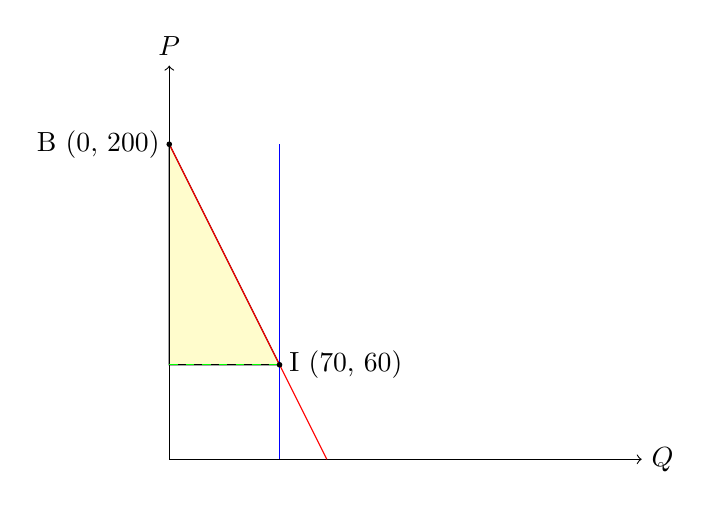
\begin{tikzpicture}
          \draw [->] (0,0) -- (6,0)node[right] {$Q$};
          \draw [->] (0,0) -- (0,5)node[above] {$P$};


          \filldraw[fill=yellow!20, scale = 0.02] (0,200) -- (70, 60) -- (0, 60) -- cycle;

          \draw[scale = 0.02, domain=0:100, smooth, variable=\x, color=red]
          plot ({\x}, {200 -  2 *\x   });

          \draw [dashed, scale = 0.02, color=green] (0,60) -- (70, 60);
          \draw [-, scale = 0.02, color=blue] (70, 200) -- (70, 0);
          %\draw [dashed, scale = 0.05, color=red] (0, 24) -- (78, 24);
          %\draw [dashed, scale = 0.05, color=blue] (0, 34) -- (78, 34);

          \filldraw[scale = 0.02, color=black] (70, 60) circle (40pt) node[anchor=west]{I (70, 60)};
          \filldraw[scale = 0.02, color=black] (0, 200)  circle (40pt) node[anchor=east]{B (0, 200)};

        \end{tikzpicture}

        thay Q = 70 vào phương trình cầu ta có P = 60 vậy giá là 60 \\
        CS là diện tích nằm trên giá và dưới đường cầu, \\
         vậy CS = (200 - 60) * 70 / 2\\
        do đường cung song song với trục tung nên chúng ta không tính được PS

  \item Tính hệ số co giãn của cầu tại mức giá này. Bạn có nhận xét gì về thu nhập của
        người trồng táo năm nay so với năm trước.

        ta viết lai phương trình đường cầu $ Q_D = 100 - 1/2P$ \\
        $P = 200 - 2Q_D$

         ta có công thức tính hệ số co giãn của cầu tại điểm như sau

         \[ E_{DP} = \frac{\%\Delta Q_D}{\%\Delta P} =
         \frac{\Delta Q_D}{\Delta P} \times \frac{P}{Q_D} = Q_D' \times \frac{P}{Q_D} \]

         $E_{DP} = -2 \times \frac{60}{70} = -1.714$\\
         giá trị tuyệt đối của $E_{DP}$ lớn hơn 1, do đó cầu co giãn theo giá 


  \item Để đảm bảo thu nhập cho người trồng táo chính phủ ấn định mức giá sàn năm nay
        là 70 nghìnđ/kg và cam kết hứa mua hết phần lúa dư thừa thì số tiền chính phủ phải
        chi ra là bao nhiêu?

        \begin{tikzpicture}
          \draw [->] (0,0) -- (6,0)node[right] {$Q$};
          \draw [->] (0,0) -- (0,5)node[above] {$P$};


          %\filldraw[fill=yellow!20, scale = 0.02] (0,200) -- (70, 60) -- (0, 60) -- cycle;

          \draw[scale = 0.02, domain=0:100, smooth, variable=\x, color=red]
          plot ({\x}, {200 -  2 *\x   });

          %\draw [dashed, scale = 0.02, color=violet] (0,60) -- (70, 60);
          \draw [-, scale = 0.02, color=blue] (70, 200) -- (70, 0);
          \draw [dashed, scale = 0.02, color=green] (0, 70) -- (70, 70);
          %\draw [dashed, scale = 0.05, color=blue] (0, 34) -- (78, 34);

          \filldraw[scale = 0.02, color=black] (70, 70) circle (40pt) node[anchor=west]{I (70, 70)};
          \filldraw[scale = 0.02, color=black] (0, 200)  circle (40pt) node[anchor=east]{B (0, 200)};
          \filldraw[scale = 0.02, color=black] (65, 70)  circle (40pt) node[anchor=north]{A (65, 70)};

        \end{tikzpicture}

        tại mức giá P = 70, giao của nó với đường cầu tại A(65, 70)\\
        điều đó có nghĩa là thị trường chỉ mua 65 tấn, còn dư 70 - 65 = 5 tấn\\
        chính phủ sẽ thu mua với giá 70 vậy số tiền chi ra là 70 * 5 = 350

  \item Nếu chính phủ đánh thuế mỗi kg táo mà người tiêu dùng mua là 5 nghìn đồng, thì
        giá cả cân bằng và sản lượng cân bằng thay đổi thế nào? Ai là người chịu thuế? Giải
        thích ?

        ở đây cung không đổi , ta có thể hiểu đó là đánh vào người mua, đường càu dịch chuyển chuyển xuống dưới
        1 khoảng đúng bằng
        mức thuế t theo như 6.2.2\\
        ta có phương trình cầu cũ $P = 200 - 2Q_D$ \\
        thuế đánh 5 nghìn đồng thì đường cầu mới sẽ là \\
        $P + 5 = 200 - 2Q_D$  ở đâu lượng cầu không đổi nhưng giá tăng thêm 5 đơn vị\\
        $P = 195 - 2Q_D$

        giá cân bằng sẽ là $P = 195 - 2 * 70 = 55$ vì sản lượng là không đổi


        \begin{tikzpicture}
          \draw [->] (0,0) -- (8,0)node[right] {$Q$};
          \draw [->] (0,0) -- (0,8)node[above] {$P$};


          %\filldraw[fill=yellow!20, scale = 0.02] (0,200) -- (70, 60) -- (0, 60) -- cycle;

          \draw[scale = 0.1, domain=60:100, smooth, variable=\x, color=black]
          plot ({\x}, {200 -  2 *\x   });

          \draw[scale = 0.1, domain=60:100, smooth, variable=\x, color=red]
          plot ({\x}, {195 -  2 *\x   });

          %\draw [dashed, scale = 0.02, color=violet] (0,60) -- (70, 60);
          \draw [-, scale = 0.1, color=blue] (70, 100) -- (70, 0);
          \draw [dashed, scale = 0.1, color=black] (0, 60) -- (70, 60);
          \draw [dashed, scale = 0.1, color=blue] (0, 55) -- (70, 55);

         \filldraw[scale = 0.1, color=black] (0, 60) circle (10pt) node[anchor=east]{P \& $P_D$};
         \filldraw[scale = 0.1, color=black] (0, 55)  circle (10pt) node[anchor=east]{$P_S$};
         % \filldraw[scale = 0.02, color=black] (65, 70)  circle (40pt) node[anchor=north]{A (65, 70)};

        \end{tikzpicture}

        chúng ta có thể nhìn thấy, sau khi đánh thuế, đường cầu dịch chuyển sang trái, do cung không đổi nên $P_S$ giảm xuống trong khi $P_D$ giữ nguyên, đo đó người bán đang bị đánh thuế\\
        điều này cũng thể hiện trong mục 6.2.3 Hệ số co giãn và sự phân chia 
        gánh nặng thuế

\end{enumerate}
\chapter{ĐO LƯỜNG THU NHẬP VÀ 
TĂNG TRƯỞNG KINH TẾ}

\section{ Các giả định sau đây ảnh hưởng như thế nào đến các thành tố của GDP theo 
cách tiếp cận chi tiêu và GDP thay đổi như thế nào.}
\begin{enumerate}[a.]
    \item 1 sinh viên Việt Nam mua 1 chiếc Wave của Honda Việt Nam.
    \item Honda Việt Nam bán 1 chiếc Dream cho một công dân Lào.
    \item Một người tiêu dùng Việt Nam mua một chiếc xe honda PCX nhập khẩu từ Thái 
    Lan
    \item Sở công an Hà Nội mua một chiếc ô tô của Honda Việt Nam.
    \item Petro Việt Nam mua một chiếc ô tô của Honda Việt Nam.
    \item Honda Việt Nam chuyển một chiếc ô tô sản xuất chiều ngày 31/12/2017 vào kho.
    10
    \item Ngày 1/1/2018 Honda Việt Nam lấy chiếc ô tô của câu e ra bán cho người tiêu 
    dùng.
\end{enumerate}

\section{ Một nền kinh tế chỉ sản xuất bút và sách có thông tin như sau. Năm gốc là năm
  2008 }

\begin{tabular}{|c|c|c|c|c|}
  \hline
  Năm  & Giá bút     & Lượng bút & Giá sách      & Lượng sách  \\
       & (1000Đ/cái) & (1000cái) & (1000Đ/quyển) & (1000quyển) \\
  \hline
  2008 & 3           & 100       & 10            & 50          \\
  \hline
  2009 & 3           & 120       & 12            & 70          \\
  \hline
  2010 & 4           & 120       & 14            & 70          \\
  \hline
\end{tabular}

\begin{enumerate}[a.]
  \item  Tính GDP danh nghĩa và GDP thực tế, chỉ số điều chỉnh GDP của các năm.

        ta có các công thức như sau:
        $$ GDP^t_n = \sum^{i}_{i = 1} q^t_i  * p^t_i $$
        n : nominal  $\Rightarrow$ danh nghĩa
        $$ GDP^t_r = \sum^{i}_{i = 1} q^t_i  * p^0_i $$
        r: real $\Rightarrow$ thực tế
        $$D^t_{GDP} = \frac{GDP^t_n}{GDP^t_r} \times 100$$
        cụ thể tính như sau\\
        $GDP^{2008}_n = 3 * 100 + 10 * 50 = 800$ \\
        $GDP^{2009}_n = 3 * 120 + 12 * 70 = 1200$ \\
        $GDP^{2010}_n = 4 * 120 + 14 * 70 = 1460$ \\
        \\
        $GDP^{2008}_r = 3 * 100 + 10 * 50 = 800$ \\
        $GDP^{2009}_r = 3 * 120 + 10 * 70 = 1060$ \\
        $GDP^{2010}_r = 3 * 120 + 10 * 70 = 1060$ \\
        \\
        $D^{2008}_{GDP} = \frac{GDP^{2008}_n}{GDP^{2008}_r} \times 100 = 100$ \\
        $D^{2009}_{GDP} = \frac{GDP^{2009}_n}{GDP^{2009}_r} \times 100 = 120/106 * 100$ \\
        $D^{2010}_{GDP} = \frac{GDP^{2010}_n}{GDP^{2010}_r} \times 100 = 146 / 106 * 100$ \\


  \item Tính tốc độ tăng trưởng kinh tế của năm 2009 và 2010. \\
        Tốc độ tăng trưởng của nền kinh tế ( GDP growth
        rate – g ) là tỷ lệ \% thay đổi của GDP thực tế từ thời
        kỳ/ năm này so với thời kỳ/ năm trước
        $$g^t = \frac{GDP^{t}_r - GDP^{t - 1}_r}{GDP^{t - 1}_r} \times 100  $$
        đơn giản thay vào công thức ta sẽ có 
        $$g^t = \frac{1060 - 1060}{1060} \times 100 = 0 $$
\end{enumerate}

\section{  Cho bảng số liệu sau, Tính tốc độ tăng trưởng kinh tế năm 2009 và 2010 }

\begin{tabular}{|c|c|c|}
  \hline
  Năm  & GDP danh nghĩa (Tỷ USD) & Chỉ số điều chỉnh GDP \\
  \hline
  2008 & 17                      & 100                   \\
  \hline
  2009 & 25                      & 118                   \\
  \hline
  2010 & 32                      & 135                   \\
  \hline
\end{tabular}

ta có công thức
$$g^t = \frac{GDP^{t}_r - GDP^{t - 1}_r}{GDP^{t - 1}_r} \times 100  $$
và
$$D^t_{GDP} = \frac{GDP^t_n}{GDP^t_r} \times 100$$
ta đang cần GDP thực tế của mỗi năm nên ta cần biến đổi công thức 
$$D^t_{GDP} = \frac{GDP^t_n}{GDP^t_r} \times 100 \Rightarrow GDP^t_r = \frac{GDP^t_n}{D^t_{GDP}} \times 100$$
từ đó 
ta có \\
$GDP^{2008}_r = \frac{GDP^{2008}_n}{D^{2008}_{GDP}} \times 100 = 17$\\
$GDP^{2009}_r = \frac{GDP^{2009}_n}{D^{2009}_{GDP}} \times 100 = 100 * 25 / 118$\\
$GDP^{2010}_r = \frac{GDP^{2010}_n}{D^{2010}_{GDP}} \times 100 = 100 * 32 / 135$

từ đó có thể tính tốc độ tăng trưởng kinh tế năm 2009 và 2010

$$g^t = \frac{GDP^{2010}_r - GDP^{2009}_r}{GDP^{2009}_r} \times 100  $$
$$g^t = \frac{100 * 32 / 135 - 100 * 25 / 118}{100 * 25 / 118} \times 100  $$
$$g^t = \frac{ 32 / 135 -  25 / 118}{25 / 118} \times 100  $$
$$g^t = \frac{ (32 * 118 - 25 * 135) / (135 * 118)}{25 / 118} \times 100  $$
$$g^t = \frac{ (32 * 118 - 25 * 135) }{ 135 * 25} \times 100  $$
\chapter{LẠM PHÁT VÀ
  THẤT NGHIỆP}

  \section{ Một nền kinh tế chỉ sản xuất 2 loại hàng tiêu dùng là lương thực và quần áo có
  số liệu như sau: (năm 2008 là năm gốc)}

\begin{tabular}{|c|c|c|c|c|}
  \hline
  Năm  & Giá lương & Lượng      & Giá quần & Lượng quần \\
       & thực      & lương thực & áo       & áo         \\
       & (1000Đ)   & (tấn)      & (1000Đ)  & (bộ)       \\
  \hline
  2008 & 2         & 100        & 1        & 100        \\
  \hline
  2009 & 2,5       & 90         & 0,9      & 120        \\
  \hline
  2010 & 2,75      & 105        & 1        & 130        \\
  \hline
\end{tabular}

\begin{enumerate}[a.]
  \item Tính CPI của các năm. \\
        ta có công thức
        $$CPI^t = \frac{\sum^{n}_{i=1}p^t_i * q^0_i}{\sum^{n}_{i=1}p^0_i * q^0_i} \times 100$$

        $CPI^{2008} = \frac{2 * 100 + 1 * 100}{2 * 100 + 1 * 100} \times 100 = 100$\\
        $CPI^{2009} = \frac{2.5 * 100 + 0.9 * 100}{2 * 100 + 1 * 100} \times 100 = \frac{340}{300}  \times 100 = 113 $\\
        $CPI^{2010} = \frac{2.75 * 100 + 1 * 100}{2 * 100 + 1 * 100} \times 100 = \frac{375}{300}  \times 100 = 125 $\\

  \item  Tính tỷ lệ lạm phát của năm 2009 và 2010.
        $$\Pi^t = \frac{CPI^t - CPI^{t -1}}{CPI^{t -1}} \times 100$$
        $$\Pi^{2009} = \frac{113 - 100}{100}  \times 100$$
        $$\Pi^{2010} = \frac{125 - 113}{113}  \times 100$$

  \item  Tính GDP danh nghĩa, GDP thực tế và chỉ số điều chỉnh GDP của các năm? Tính tỉ lệ lạm phát của năm 2009 và 2010 theo chỉ số điều chỉnh GDP \\
        ta có công thức\\
        Tốc độ tăng trưởng của nền kinh tế
        $$g^t = \frac{GDP^{t}_r - GDP^{t - 1}_r}{GDP^{t - 1}_r} \times 100  $$
        và        
        $$ GDP^t_n = \sum^{i}_{i = 1} q^t_i  * p^t_i $$
        n : nominal  $\Rightarrow$ danh nghĩa
        $$ GDP^t_r = \sum^{i}_{i = 1} q^t_i  * p^0_i $$
        r: real $\Rightarrow$ thực tế\\
        Chỉ số điều chỉnh GDP
        $$D^t_{GDP} = \frac{GDP^t_n}{GDP^t_r} \times 100$$

        $$ GDP^{2008}_n = 2 * 100 +1 * 100 = 300 $$
        $$ GDP^{2009}_n = 2.5 * 90 + 0.9 * 120 = 225 + 108 = 313 $$
        $$ GDP^{2010}_n = 2.75 * 105 + 1 * 130 = 288.75 + 130 = 418.75 $$

        $$ GDP^{2008}_r = 2 * 100 + 1 * 100 = 300 $$
        $$ GDP^{2009}_r = 2 * 90 + 1 * 120 = 180 + 120 = 300 $$
        $$ GDP^{2010}_r = 2 * 105 + 1 * 130 = 210 + 130 = 340 $$

        $$D^{2008}_{GDP} = \frac{300}{300} \times 100$$
        $$D^{2009}_{GDP} = \frac{313}{300} \times 100$$
        $$D^{2010}_{GDP} = \frac{418.75}{340} \times 100$$ 
        để tính tỷ lệ lạm phát chúng ta cần biết CPI\\
        vậy ta càn tìm sự liên hệ gữa CPI và D "chỉ số điều chỉnh"\\
        $$D^t_{GDP} = \frac{GDP^t_n}{GDP^t_r} \times 100 \Rightarrow \frac{100}{D^t_{GDP}} = \frac{GDP^t_r}{GDP^t_n} \Rightarrow \frac{100 * GDP^t_n}{D^t_{GDP}} = GDP^t_r $$
        $CPI^t = \frac{\sum^{n}_{i=1}p^t_i * q^0_i}{\sum^{n}_{i=1}p^0_i * q^0_i} \times 100 = \frac{GDP^t_r}{GDP^0_r}  \times 100 $\\
        \[\Pi^t = \frac{CPI^t - CPI^{t -1}}{CPI^{t -1}} \times 100 = \frac{\frac{GDP^t_r}{GDP^0_r} - \frac{GDP^{t-1}_r}{GDP^0_r}}{\frac{GDP^{t-1}_r}{GDP^0_r}} \times 100 = \frac{GDP^t_r - GDP^{t-1}_r}{GDP^{t-1}_r} \times 100\]
        $ = \frac{GDP^t_r}{GDP^{t-1}_r} \times 100 - 100 = \frac{GDP^t_n * D^{t-1}_{GDP}}{D^t_{GDP}* GDP^{t-1}_n} \times 100 - 100$\\
        $ = \frac{GDP^t_n * D^{t-1}_{GDP} - D^t_{GDP}* GDP^{t-1}_n }{D^t_{GDP}* GDP^{t-1}_n} \times 100$


\end{enumerate}


\section{Tại năm 2007, một người có mức thu nhập là 150 triệu đồng/năm.}
Tại năm 2007, một người có mức thu nhập là 150 triệu đồng/năm. Năm 2017 thu nhập 
của anh ta là 255 triệu đồng/năm. Biết CPI năm 2007 là 112 và CPI năm 2017 là 168. Vậy tại 
năm 2017 người này được xem là có mức sống cao hơn, thấp hơn hay tương đương với năm 
2007?

Để làm bài này chúng ta xem lại 8.1.5. Điều chỉnh các biến số kinh tế 
theo lạm phát.\\
theo đó ta tính như sau\\
thu nhập năm 2017 tính theo 2007 = thu nhập 2007 * ($CPI_{2017}/CPI_{2007}$)\\
$= 150 * 168 / 112 = 225$\\
vậy người này có mức sống cao hơn

Lãi suất danh nghĩa là 7$\%$/năm, tỉ lệ lạm phát là 3\%/năm. Mức thuế suất đánh vào 
thu nhập từ tiền lãi là 10\%. Tính lãi suất thực tế sau thuế?

theo 8.1.5. Điều chỉnh các biến số kinh tế 
theo lạm phát chúng ta có \\
- Lãi suất danh nghĩa (nominal interest rate – i)  \\
- Lãi suất thực tế (real interest rate – r) \\
- lãi suất thực tế mới là cái thực sự được quan tâm \\
$$r = i - \pi$$
và theo nội dung của slide "Tác hại của lạm phát ( tiếp)"\\ 
chúng ta có bảng sau\\
\begin{tabular}{|l|r|}
  \hline
  Lãi suất danh nghĩa(nominal interest: i) & 7\% \\
  \hline
Tỷ lệ lạm phát ($\pi$ ) & 3\% \\
\hline
Lãi suất thực tế (real interest: r = i – $\pi$) & 4\% \\
\hline
Thuế (10\%* i) & 0.7\%\\
\hline
Lãi suất danh nghĩa sau thuế &   7\% - 0.7\% = 6.3\% \\
$i_{\textmd{sau thuế}} = i - 10\%*i$ & \\
\hline
Lãi suất thực tế sau thuế & 6.3\% - 3\% = 3.3\% \\
$r_{\textmd{sau thuế}} = i_{\textmd{sau thuế}} - \pi$ & \\
\hline
\end{tabular}

\section{. Vào thời điểm ngày 1/7/2004 tai một nước A,}
Vào thời điểm ngày 1/7/2004 tai một nước A, tổng dân số nước A là 82 triệu người, 
số người có việc làm là 41,6 triệu người, số người thất nghiệp là 0,9 triệu người. Số người 
ngoài độ tuổi lao động chiếm 45 \% dân số. Hãy tính:
\begin{enumerate}[-]
  \item Số người trong độ tuổi lao động \\
  = tổng dân số - Số người ngoài độ tuổi lao động = 82 - 0.45 * 82 = 45.1  
  \item Tỉ lệ tham gia lực lượng lao động \\
  Tỷ lệ tham gia lực lượng lao động = (lực lượng lao động / tổng số người trưởng thành)*100\% \\
  = (số người có việc làm + số người thất nghiệp) / Số người trong độ tuổi lao động * 100\% \\
  = (41.6 + 0.9) / 45.1 * 100\% = 42.5 / 45.1 * 100\% =  94.235\% = 94.23\%
  \item Tỉ lệ thất nghiệp \\
  Tỷ lệ thất nghiệp = (số người thất nghiệp / lực 
lượng lao động)*100\%. \\
  = 0.9 / 45.1 *100\% = 1.99556541\%  $\approx$ 1.995\% $\approx$ 1.99\%
  \item Tỷ lệ người có việc làm \\
  Tỷ lệ người có việc làm = (người có việc làm/ lực 
lượng lao động)*100\% \\
  = 41.6 / 45.1 *100\% = 92.23946784\% $\approx$ 92.24 \%
\end{enumerate}


\chapter{TIẾT KIỆM, ĐẦU TƯ VÀ 
HỆ THỐNG TÀI CHÍNH}

\setcounter{section}{1}
\section{Một nền kinh tế đóng có GDP là 1000 tỷ đồng}
Một nền kinh tế đóng có GDP là 1000 tỷ đồng, thuế là 150 tỷ đồng, tiết kiệm tư 
nhân là 250 tỷ đồng, tiết kiệm chính phủ là -30 tỷ đồng. Hãy tính tiêu dùng của hộ gia 
đình, chi tiêu của chính phủ, tiết kiệm quốc dân và đầu tư.\\
đầu tiên chúng ta ta lưu ý rằng đây là 1 nên kinh tế đóng \\
và có công thức như sau\\
$Y = C + I + G$ với $I = Y - C - G = S_n $ là tiết kiệm quốc dân\\
và trong nền kinh tế đóng Tiết Kiệm = đầu tư\\
Y: GDP. \\
C: Chi cho tiêu dùng cá nhân của các hộ gia đình về hàng hóa và dịch vụ \\
I: Đầu tư phán ánh tổng đầu tư trong nước của khu vực tư nhân \\
G: chi tiêu cho các cấp chính quyền từ trung ương tới địa phương.\\
T:  tổng số tiền thuế mà chính phủ thu được sau 
khi trừ đi các khoản trợ cấp hoặc chuyển giao thu nhập \\
Y - T - C: tiết kiệm tư nhân\\
T - G: tiếp kiệm chính phủ\\
Cán cân ngân sách (B) B = T - G

chúng ta đang có T - G = -30, T = 150, Y - T - C = 250, Y = 1000\\
vậy \\
tiêu dùng của hộ gia đình = C = Y - T -250 = 1000 - 150 - 250 = 600\\
chi tiêu của chính phủ = G = T + 30 = 150 + 30 = 180\\
tiết kiệm quốc dân = đầu tư = Y - C - G = 1000 - 600  - 180 = 280





\end{document}